\documentclass[12pt,a4paper]{report}

\usepackage[T1]{fontenc}
\usepackage[utf8]{inputenc}
\usepackage[margin=1in]{geometry}
\usepackage{setspace}
\usepackage{graphicx}
\graphicspath{{figures/}}
\usepackage{xcolor}
\usepackage{tikz}
\usetikzlibrary{arrows.meta,positioning}
% Colours and dimensions for TikZ figures (data in figures/data/)
\definecolor{benignblue}{HTML}{4C78A8}
\definecolor{malwarered}{HTML}{E45756}
\definecolor{uncertainorange}{HTML}{F58518}
\definecolor{certaingreen}{HTML}{72B7B2}
\definecolor{familygreen}{HTML}{54A24B}
\definecolor{verdictpurple}{HTML}{B279A2}
\def\TikzBarWidth{1.1}
\def\TikzBarUnit{0.22}

% TikZ helpers — confusion matrix uses \CmTN, \CmFP, \CmFN, \CmTP from values_*.tex

\newcommand{\TikzConfusionMatrix}{%
  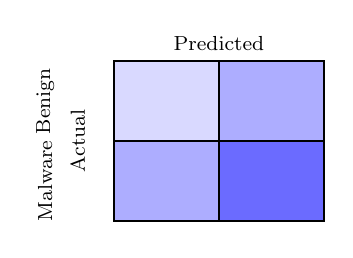
\begin{tikzpicture}[scale=0.92, transform shape,
    font=\small,
    cell/.style={minimum width=1.35cm, minimum height=1.0cm, align=center, inner sep=2pt},
    lbl/.style={font=\footnotesize, align=center},
  ]
  \node[lbl] at (1.45, 2.45) {Predicted};
  \node[lbl] at (0.725, 2.05) {Benign};
  \node[lbl] at (2.175, 2.05) {Malware};
  \node[lbl, rotate=90] at (-0.5, 1.1) {Actual};
  \node[lbl, rotate=90] at (-0.95, 1.65) {Benign};
  \node[lbl, rotate=90] at (-0.95, 0.55) {Malware};
  \fill[blue!15] (0,1.1) rectangle (1.45,2.2);
  \fill[blue!32] (1.45,1.1) rectangle (2.9,2.2);
  \fill[blue!32] (0,0) rectangle (1.45,1.1);
  \fill[blue!58] (1.45,0) rectangle (2.9,1.1);
  \node[cell, font=\small\bfseries] at (0.725, 1.65) {\CmTN};
  \node[cell, font=\small\bfseries] at (2.175, 1.65) {\CmFP};
  \node[cell, font=\small\bfseries] at (0.725, 0.55) {\CmFN};
  \node[cell, font=\small\bfseries] at (2.175, 0.55) {\CmTP};
  \draw[thick] (0,0) rectangle (2.9,2.2);
  \draw (1.45,0) -- (1.45,2.2);
  \draw (0,1.1) -- (2.9,1.1);
  \end{tikzpicture}%
}

% Map raw count to y (cm); axis spans [ymin, ymax] on log10 scale, plotted height \plotH cm.
\newcommand{\TikzCountY}[4]{%
  \pgfmathsetmacro{#4}{(ln(max(#1,1))/ln(10) - ln(max(#2,1))/ln(10)) / (ln(max(#3,1))/ln(10) - ln(max(#2,1))/ln(10))}%
}

\newcommand{\TikzLogStrip}[6]{%
  % #1=x centre, #2=colour, #3=macro with comma list, #4=ymin #5=ymax #6=plot height (cm)
  \foreach \v [count=\i] in #3 {
    \TikzCountY{\v}{#4}{#5}{\yraw}
    \pgfmathsetmacro{\y}{\yraw * #6}
    \pgfmathsetmacro{\dx}{mod(\i-1,2)==0 ? 0.08 : -0.08}
    \fill[#2] (#1+\dx,\y) circle (1.6pt);
  }%
}

\newcommand{\TikzLogAxis}[5]{%
  % #1=x0 #2=x1 #3=ymin #4=ymax #5=plot height (cm)
  \foreach \t/\lbl in {2/100,3/1k,4/10k,5/100k} {
    \pgfmathparse{and(10^\t >= #3, 10^\t <= #4)}
    \ifnum\pgfmathresult=1
      \TikzCountY{10^\t}{#3}{#4}{\yraw}
      \pgfmathsetmacro{\y}{\yraw * #5}
      \draw[gray!55] (#1,\y) -- (#2,\y);
      \node[font=\footnotesize, anchor=east] at (#1-0.08,\y) {\lbl};
    \fi
  }%
}

\newcommand{\TikzTriageBars}[1]{%
  % #1 = max count for bar width scaling
  \pgfmathsetmacro{\barW}{9.2/max(#1,1)}
  \foreach \lbl/\cnt [count=\i] in \BarRows {
    \pgfmathsetmacro{\y}{(\i-1)*0.95}
    \draw[fill=benignblue!75, draw=black!60, line width=0.3pt]
      (0,\y) rectangle ({\cnt*\barW},\y+0.72);
    \node[anchor=west, font=\small] at (0.14,\y+0.36) {\lbl};
    \node[anchor=east, font=\small\bfseries] at ({\cnt*\barW}-0.14,\y+0.36) {\cnt};
  }%
}

\usepackage{microtype}
\hyphenation{artefacts malware forensics Volatility heterogeneous}
\usepackage{booktabs}
\usepackage{caption}
\usepackage{subcaption}
\usepackage{longtable}
\usepackage{array}
\usepackage{tabularx}
\usepackage{cite}
\usepackage{xurl}
\usepackage{listings}
\lstset{
  basicstyle=\ttfamily\footnotesize,
  breaklines=true,
  breakatwhitespace=true,
  columns=fullflexible,
  keepspaces=true,
  showstringspaces=false,
  frame=single,
  framerule=0.4pt,
  literate={_}{\textunderscore}1
}
\usepackage{hyperref}

\hypersetup{
  colorlinks=true,
  linkcolor=black,
  citecolor=black,
  urlcolor=blue,
  pdftitle={Graph-Based Deep Learning for Malware Detection Using Windows Memory Forensics},
  pdfauthor={VIRAJ RAJESHBHAI CHUDASAMA}
}

\onehalfspacing
\setcounter{tocdepth}{2}

\begin{document}

\begin{titlepage}
\centering
\vspace*{2cm}
{\Large \textbf{Graph-Based Deep Learning for Malware Detection Using Windows Memory Forensics}\par}
\vspace{2cm}
{\large \textbf{Name:} VIRAJ RAJESHBHAI CHUDASAMA\par}
\vspace{0.3cm}
{\large \textbf{Supervisor:} Mohamed Ghanem\par}
\vspace{0.3cm}
{\large \textbf{Programme:} MSc Cyber Security\par}
\vspace{0.3cm}
{\large \textbf{Date:} May 2026\par}
\vfill
\end{titlepage}

\chapter*{Declaration}
\addcontentsline{toc}{chapter}{Declaration}
I declare that this project is my own work and has been prepared in line with the rules and guidance of the University of Wales Trinity Saint David.

\vspace{1cm}
\noindent Signed: \rule{7cm}{0.4pt}

\vspace{0.6cm}
\noindent Date: \rule{7cm}{0.4pt}

\chapter*{Abstract}
\addcontentsline{toc}{chapter}{Abstract}
Malware often hides in live memory, while file-based scanning can miss injection, covert processes, and short-lived network activity. Windows memory forensics captures processes, DLLs, memory regions, handles, and network objects at capture time, but Volatility plugin output is large and difficult to compare across samples by hand.

This dissertation implements a proof-of-concept pipeline: Volatility~3 artefacts are converted into typed memory-snapshot graphs, scored by graph neural networks (GIN, GraphSAGE, GAT, GINE), and explained with structured evidence and uncertainty fields. A hybrid rule layer supplies graph attributes and triage verdicts; binary and two-model paths support analyst review.

The central empirical finding is label--signal mismatch on benign baselines: in the current manifest ($n{=}30$), \textbf{14 of 15} benign-labelled (\texttt{NoVirus}) rows are flagged \texttt{uncertain=True} because rule-based triage still reports HIGH or CRITICAL activity (injection counts, process scores, C2-style connections). Folder names are therefore an imperfect proxy for ground truth; uncertainty must be reported, not hidden.

Contributions include a reproducible extraction-to-graph workflow, manifest governance, GNN training scripts with family-grouped cross-validation, and optional dashboard scanning. Metrics tables in Chapter~\ref{ch:evaluation} use placeholders until grouped CV is run on archived checkpoints.

\textbf{Limitation:} With $n{=}30$ graphs and noisy benign labels, the work demonstrates feasibility and evidence organisation---not production detection performance.

\vspace{0.5cm}
\noindent\textbf{Keywords:} malware detection, Windows memory forensics, Volatility 3, graph neural networks, heterogeneous graphs, PyTorch Geometric, GINE, anomaly detection, digital forensics, explainable AI

\tableofcontents
\clearpage

\chapter{Introduction}

\section{Background}

Cybercrime and cyber-enabled fraud continue to affect global economies. Malware is a core tool in many attack chains, including ransomware campaigns, credential theft, and long-term compromise. Organisations therefore invest in endpoint detection, logging, and forensic response capabilities. Despite these investments, skilled analysts remain necessary because automated tools can miss context, produce false positives, or fail on novel families.

Malware is still a major problem for organisations, universities, public services, and personal users \cite{ucci2019survey}. Modern malware does not only exist as a file on disk. It may inject code into trusted processes, load suspicious modules, communicate with remote hosts, hide process activity, or perform actions only for a short time \cite{egele2012survey}. These behaviours are often visible in memory before they are fully visible in normal file logs.

Attackers also use techniques described in public frameworks such as MITRE ATT\&CK, including process injection and impact operations \cite{mitre2026enterprise}, \cite{mitre2026t1055}. Security teams therefore need methods that can inspect live system state, not only files after the event.

Digital forensics and incident response teams use memory forensics to investigate this type of activity. Memory forensics can show active processes, terminated process traces, DLLs, network connections, command-line arguments, file handles, registry hives, and suspicious memory pages \cite{ligh2014art}. Tools such as Volatility 3 make this analysis possible in a structured way \cite{volatility3docs}. Even so, the output of many plugins can be difficult to read. A single memory dump can produce many CSV files and thousands of rows.

This project uses graph-based deep learning to improve how memory-forensics artefacts are represented and analysed. A graph is a natural format for memory evidence because operating system behaviour is relational \cite{russinovich2017internals1}. A process starts another process. A process loads a DLL. A memory region belongs to a process. A network connection is owned by a process. These relationships are important for malware detection. A flat table can store these values, but it does not show the structure as clearly as a graph.

Graph neural networks can learn from both node features and graph structure \cite{hamilton2020graph}. This makes them suitable for malware detection from memory snapshots. Instead of checking only one indicator, the model can learn patterns across process trees, memory regions, network objects, and other forensic artefacts.

\section{Motivation}

The motivation for this work comes from three practical problems seen during project development.

First, memory-forensics output is large. Analysts can spend significant time moving between plugin tables to build a mental model of one host. A graph representation can keep relationships visible in one structure.

Second, malware labels are not always clean. Benign memory snapshots may still contain suspicious indicators such as injected pages or high process scores. A detection system should report uncertainty instead of hiding it \cite{guo2017calibration}.

Third, research prototypes often lack reproducibility. Without manifests, contracts, and saved artefacts, it is hard to repeat experiments or explain a score months later \cite{goodman2016reproducibility}. This dissertation therefore treats the pipeline and dataset manifest as core research outputs, not only the model weights.

\section{Problem Statement}

The main problem is that Windows memory forensics produces rich evidence, but this evidence is hard to scale, compare, and interpret manually. Analysts can run Volatility plugins, but they still need to connect many separate outputs into one clear view of behaviour. This becomes harder when there are many samples or when the evidence is noisy.

This dissertation addresses four practical gaps:

\begin{itemize}
\item \textbf{Representation gap:} plugin outputs are usually stored as separate tables, while malware behaviour is relational.
\item \textbf{Learning gap:} many forensic workflows use rules or manual checks, but they do not learn structural patterns from complete memory snapshots.
\item \textbf{Explainability gap:} a useful detection system should give evidence, not only a malware or benign label.
\item \textbf{Reproducibility gap:} memory-forensics experiments need stable artefacts, manifests, data contracts, and repeatable commands.
\end{itemize}

\section{Research Aim}

The aim of this dissertation is to design and evaluate a graph-based deep learning pipeline for malware detection using Windows memory-forensics artefacts extracted with Volatility 3.

The work is positioned as a \textbf{proof-of-concept}: it demonstrates feasibility of graph-based memory-forensics machine learning with structured evidence and uncertainty reporting, not production-grade detection performance.

\section{Key Definitions}

For clarity, this dissertation uses the following working definitions:

\textbf{Memory snapshot graph:} a heterogeneous graph built from one memory dump's Volatility artefacts, representing system entities and relationships at capture time.

\textbf{Malware-labelled sample:} a manifest row with label 1, usually corresponding to a \texttt{WithVirus} folder.

\textbf{Benign-labelled sample:} a manifest row with label 0, usually corresponding to a \texttt{NoVirus} folder, possibly flagged uncertain.

\textbf{Evidence:} structured fields (attributes, nodes, edges, narratives) that explain why a sample received a score or triage state.

\section{Primary Expected Contribution}

The expected primary contribution is empirical and methodological rather than a new detection benchmark. On the available corpus, benign-labelled memory snapshots frequently exhibit HIGH or CRITICAL triage signals despite \texttt{NoVirus} folder names (14 of 15 benign rows marked uncertain in the manifest). This finding shows that memory-forensics labels derived from folder pairing can diverge sharply from rule-based risk signals.

The secondary contributions are engineering artefacts: a Volatility-to-graph pipeline, manifest-indexed dataset, GNN and tabular evaluation scripts with family-grouped splits, and JSON evidence fields for analyst review. Together they support reproducible feasibility studies on small memory-forensics corpora.

\section{Research Objectives}

The objectives are:

\begin{enumerate}
\item To extract Windows memory-forensics artefacts from memory dumps using Volatility 3. This includes process, memory, network, and registry-related plugin outputs stored as repeatable CSV artefacts.
\item To convert plugin outputs into typed memory-snapshot graphs with entities and relationships analysts recognise (process parentage, DLL loading, injection links).
\item To engineer node, edge, and graph-level features suitable for graph neural networks. Features must remain stable across samples so training and inference use the same contracts.
\item To train and analyse GNN-based malware detection models. The project includes binary classification and one-class conformity models for richer triage states.
\item To preserve model evidence and uncertainty so that analyst review remains possible. Outputs should include top attributes, important nodes, and short narratives.
\item To evaluate the strengths and limits of the approach using available project artefacts. Evaluation must discuss dataset size, label noise, and family overlap honestly.
\end{enumerate}

\section{Research Questions}

This project is guided by the following questions:

\begin{enumerate}
\item How can Windows memory-forensics artefacts be represented as a graph for malware detection? The answer is developed through the node and edge schema in Chapters~\ref{ch:methodology} and~\ref{ch:design}, and through graph statistics in Chapter~\ref{ch:evaluation}.
\item Which system entities and relationships are most useful for graph-based detection? The project prioritises process, memory, network, and DLL relationships, plus behaviour-intent edges aligned with common attack patterns.
\item How can GNN models support malware detection while still providing structured evidence? The binary and two-model paths combine learned scores with rule-based graph attributes and JSON evidence fields.
\item What limitations appear when graph-based learning is applied to a small memory-forensics corpus? Chapter~\ref{ch:evaluation} discusses uncertain benign rows, graph-size variation, and the risk of overconfident conclusions.
\end{enumerate}

\section{Contributions Preview}

The main contributions of this dissertation are:

\begin{itemize}
\item a Volatility~3 extraction workflow for Windows memory artefacts;
\item a heterogeneous graph schema for memory-forensics entities and relationships;
\item graph-level feature engineering linked to triage signals;
\item GNN model support for binary and one-class analysis paths;
\item structured model evidence and uncertainty reporting;
\item a dataset manifest for reproducible experiments;
\item optional dashboard integration for upload-session model scanning.
\end{itemize}

\section{Scope}

This is a writing and research project based on an implemented repository. The work focuses on Windows memory dumps, Volatility 3 artefacts, graph construction, and graph-based deep learning. The dataset includes several malware-family folders and paired NoVirus folders. Ransomware samples are included as part of the corpus, but the topic is not limited to ransomware. The correct topic is broader: graph-based deep learning for malware detection using Windows memory forensics.

The dissertation does not include malware binaries in the written submission. It discusses memory dumps only at the artefact level. Ethics and safe handling are addressed in Chapter~\ref{ch:methodology}.

\section{Dissertation Structure}

Chapter~1 introduces the problem and the research aim. Chapter~2 reviews memory forensics, malware analysis, graph learning, GNNs, anomaly detection, and explainability. Chapter~3 explains the methodology. Chapter~4 presents the system design. Chapter~5 describes the implementation. Chapter~6 discusses the results and limitations. Chapter~7 concludes the dissertation and suggests future work. Chapter~8 gives a personal reflection.

\section{Context: Memory Forensics in Incident Response}

Incident response workflows often move from live collection to disk forensics and then to memory forensics when analysts suspect hidden processes, injection, or ransomware activity \cite{nist2012sp80061}. Commercial and open-source tools can acquire RAM images, but the analysis step remains difficult at scale. Analysts must decide which processes, memory regions, and network objects deserve deeper review.

This dissertation does not replace Volatility or other forensic suites. Instead, it proposes a structured bridge between plugin outputs and machine-learning models. The bridge is a graph representation with explicit evidence fields. That design choice keeps the workflow understandable for security practitioners who may not be deep-learning specialists.

\section{Expected Outcomes}

By the end of this work, a reader should understand four outcomes:

\begin{enumerate}
\item how Windows memory artefacts are converted into heterogeneous graphs;
\item how graph features and GNN models are used for malware triage;
\item how uncertainty and evidence are reported in analysis outputs;
\item what limitations apply when the corpus is small and labels are noisy.
\end{enumerate}

These outcomes align with the research questions and support a fair interpretation of results in later chapters. Together they define what success means for this applied security project.

\chapter{Literature Review}

\section{Malware Detection}

Malware remains a persistent threat to individuals, businesses, and critical infrastructure. Attackers use packed binaries, living-off-the-land techniques, credential theft, ransomware, and memory-resident methods to evade traditional defences. Public guidance from CISA and related bodies emphasises layered detection, incident response preparation, and malware analysis tradecraft \cite{cisa2023stopransomware}, \cite{cisa2026advisories}.

Malware detection has moved from simple signature matching to more behaviour-based and learning-based approaches. Signature methods can be fast, but they often fail when malware changes its hash, packs itself, or uses obfuscation \cite{santos2009ngrams}. Behaviour-based approaches study actions such as process creation, API use, file activity, persistence, network communication, and memory injection. These methods are more useful when malware changes its surface form but keeps similar behaviour.

Christodorescu et al.\ introduced semantics-aware malware detection to reason about program meaning rather than raw bytes alone \cite{christodorescu2005semantics}. Moser et al.\ showed that static analysis alone has clear limits for packed or obfuscated malware \cite{moser2007limits}. These findings explain why modern work often combines multiple evidence layers instead of relying on one technique.

Dynamic malware analysis is useful because it observes behaviour during execution. Egele et al.\ describe how automated dynamic analysis systems can record system calls, network traffic, and other runtime events \cite{egele2012survey}. Bayer et al.\ show that malware behaviour can be clustered and compared using runtime profiles \cite{bayer2009scalable}. Willems et al.\ discuss automated dynamic malware analysis using sandbox environments \cite{willems2007cwsandbox}. Yin et al.\ present Panorama, which captures system-wide information flow for malware detection and analysis \cite{yin2007panorama}. These ideas support the approach used in this dissertation because memory forensics also studies runtime state.

However, dynamic analysis can be limited by sandbox evasion, environment differences, and incomplete execution. Memory forensics gives a different evidence layer. It can capture live runtime objects and artefacts that may not exist on disk. This is useful for malware that hides itself or runs only in memory.

Ucci et al.\ provide a broad survey of machine learning techniques for malware analysis \cite{ucci2019survey}. Their review shows that feature design, label quality, and evaluation design are often more important than the choice of classifier. This dissertation follows that lesson by focusing on graph representation and reproducible artefacts before claiming strong detection performance.

\section{Static, Dynamic, and Memory-Based Analysis}

Table~\ref{tab:analysis_comparison} compares three common analysis layers. Each layer has strengths, but none is sufficient alone for difficult malware cases.

\begin{table}[htbp]
\centering
\caption{Comparison of malware analysis layers relevant to this project.}
\label{tab:analysis_comparison}
\begin{tabular}{p{2.2cm}p{3.2cm}p{2cm}p{2.2cm}p{3.2cm}}
\toprule
\textbf{Layer} & \textbf{Typical data} & \textbf{Uses graph?} & \textbf{Explainability} & \textbf{Main limitation} \\
\midrule
Static & Bytecode, CFG, API calls & Often & Medium & Packing and obfuscation \\
Dynamic & Syscalls, files, network & Sometimes & Medium & Sandbox evasion \\
Memory & Processes, VAD, sockets & Rare in prior work & High potential & Noisy baselines, scale \\
\bottomrule
\end{tabular}
\end{table}

Static analysis is efficient for known patterns, but attackers can change file structure while keeping malicious runtime behaviour. Dynamic analysis observes execution, yet it may miss behaviour that appears only in specific host states. Memory forensics captures volatile state at one point in time. Ligh et al.\ explain that memory analysis can reveal artefacts not available from disk alone \cite{ligh2014art}. This project uses memory forensics as the primary evidence source and then converts artefacts into graphs for learning.

\section{Memory Forensics}

Memory forensics is the analysis of volatile memory. It is important because memory can contain processes, handles, command lines, loaded modules, sockets, registry artefacts, injected pages, encryption keys, and other evidence. NIST recommends forensic techniques as part of incident response and evidence handling \cite{nist2006sp80086}. NIST also provides guidance for security incident handling in operational environments \cite{nist2012sp80061}.

Volatility is a common framework for memory forensics. Volatility 3 is a modern rewrite of the framework and supports many plugins for Windows, Linux, and macOS memory analysis \cite{volatility3docs}, \cite{volatility3github}. In this project, Volatility 3 is used to extract Windows artefacts such as \texttt{pslist}, \texttt{psscan}, \texttt{pstree}, \texttt{malfind}, \texttt{netscan}, \texttt{cmdline}, \texttt{dlllist}, \texttt{handles}, \texttt{threads}, \texttt{vadinfo}, \texttt{filescan}, \texttt{driverscan}, \texttt{ssdt}, and registry hive information.

Case and Richard discuss the future direction of memory forensics research and highlight the need for scalable, repeatable workflows \cite{case2017memory}. Garfinkel also argues that digital forensics research must improve reproducibility and validation over the next decade \cite{garfinkel2010digital}. These points motivate the manifest-based pipeline used in this dissertation.

Memory forensics is not simple. Symbol tables, plugin differences, large dump sizes, and noisy outputs can affect results. Therefore, this project includes a pipeline that stores outputs, checks artefacts, builds graphs, and records dataset-level metadata.

Analysts must also understand acquisition effects. A memory image captured too late may miss short-lived processes. An image captured during heavy system load may contain many benign artefacts that look suspicious in isolation. These practical constraints are one reason why graph-level uncertainty reporting is included in the project design.

Compared with disk forensics, memory forensics is closer to runtime behaviour. Compared with sandbox logs, memory forensics can show state that malware tried to hide after execution. The dissertation uses this middle layer as the primary evidence source because it matches the project's Windows memory dump data.

\section{Windows Memory Artefacts and Internals}

Windows is a widely deployed operating system with complex kernel and user-mode internals. Forensic analysts commonly examine processes, threads, VAD trees, loaded modules, network connections, and kernel structures when investigating compromise. The Volatility plugin set used in this project reflects common investigative questions: what was running, what was connected, what was injected, and what kernel objects were present at capture time.

Windows memory contains many object types that are useful for malware detection. Process lists show visible processes. Pool scans can show hidden or terminated process traces. Command-line artefacts can show suspicious execution. DLL lists can show unusual module loading. Memory regions can show executable or writable pages. Network scans can show active connections. Handles can show process ownership and access behaviour.

Russinovich et al.\ describe Windows internals in detail, including process management, memory management, and I/O subsystems \cite{russinovich2017internals1}, \cite{russinovich2021internals2}. Microsoft documentation also provides practical reference material for analysts \cite{microsoft2026windowsinternals}. This background helps explain why memory snapshots contain rich relational structure rather than isolated records.

The important point is that these artefacts are connected. A suspicious process may have injected memory, unusual DLL paths, many handles, and network activity. A graph can join these signals into one structure. This is why the dissertation uses graph construction instead of only table-based analysis.

Graziano et al.\ study hypervisor memory forensics and show that memory analysis can extend beyond standard host snapshots \cite{graziano2013hypervisor}. Although this project focuses on Windows user-mode and kernel artefacts from standard dumps, that work supports the broader claim that memory evidence remains central in advanced threat analysis.

\section{Standards, Frameworks, and Incident Response Context}

Digital investigations must follow sound evidence handling. ISO/IEC 27037 provides guidelines for identification, collection, acquisition, and preservation of digital evidence \cite{iso2012digital}. Casey discusses digital evidence and computer crime from a forensic science perspective \cite{casey2011digital}. Carrier provides detailed file system forensic analysis methods \cite{carrier2005filesystem}. These sources do not define malware models directly, but they justify careful artefact management in this project.

The MITRE ATT\&CK framework documents adversary tactics and techniques in a structured way \cite{mitre2026enterprise}. Techniques such as process injection (T1055) and data encrypted for impact (T1486) are relevant to memory-forensics findings \cite{mitre2026t1055}, \cite{mitre2026t1486}. The project maps some graph edge types to these ideas so that model inputs are easier to interpret during analyst review.

\section{Graph Representation Learning}

Graphs are used when relationships are as important as individual records. In a graph, nodes represent entities and edges represent relationships. Graph representation learning tries to learn useful vector representations from graph structure and node attributes. Hamilton gives a broad introduction to graph representation learning and its use in machine learning \cite{hamilton2020graph}.

Before GNNs became common, methods such as DeepWalk and node2vec learned embeddings from random walks on graphs \cite{perozzi2014deepwalk}, \cite{grover2016node2vec}. Mikolov et al.\ introduced efficient word embedding methods that influenced later graph embedding work \cite{mikolov2013word}. These methods show that structure can be converted into vectors, but they do not always use node attributes or edge types as flexibly as modern GNNs.

Graph neural networks extend deep learning to graph data. Kipf and Welling introduced a graph convolutional network for semi-supervised learning on graphs \cite{kipf2017gcn}. Hamilton, Ying, and Leskovec introduced GraphSAGE, which learns inductive node representations by aggregating neighbourhood information \cite{hamilton2017graphsage}. Velickovic et al.\ introduced graph attention networks, where attention weights are used for neighbouring nodes \cite{velickovic2018gat}. Xu et al.\ introduced the Graph Isomorphism Network and studied the expressive power of GNNs \cite{xu2019gin}. Fey and Lenssen describe practical graph learning with PyTorch Geometric \cite{fey2019pyg}. These models support the idea that structure can improve learning.

This project uses GNN ideas for graph-level malware detection. The model does not classify one node only. It scores the whole memory snapshot graph.

\subsection{Message passing intuition}

In message-passing GNNs, each node updates its representation using messages from neighbours. After several layers, a node representation can reflect multi-hop structure. For memory graphs, this means a process node can be influenced by connected memory regions, DLLs, and network objects. Graph-level pooling then aggregates node information into a snapshot-level embedding.

The choice of backbone involves trade-offs. GIN is strong for discriminative graph classification. GraphSAGE supports inductive settings. GAT adds attention weights to neighbours. GINE is attractive for this project because edge types are informative and should not be collapsed into unlabeled edges. The implementation therefore emphasises GINE-style models for binary and one-class paths.

\subsection{Limitations of GNNs in security applications}

GNNs are not a default win for forensic malware detection. Several structural limits apply.

\textbf{Oversmoothing and depth.} Deep message-passing stacks can make node representations indistinguishable, reducing discriminative power on large graphs \cite{rusch2023oversmoothing}, \cite{chen2022gnnsurvey}. Memory snapshots with tens of thousands of nodes are therefore sensitive to layer count and pooling choices.

\textbf{Scalability.} Full-graph training on large memory graphs is memory-intensive. Subsampling, pooling, or graph coarsening may be required, which can remove rare but important artefacts (for example a single injected region).

\textbf{Explainability gaps.} Post-hoc explainers (GNNExplainer, SHAP) help, but they do not guarantee faithful forensic narratives \cite{ying2019gnnexplainer}, \cite{lundberg2017shap}. This project mitigates the gap with rule-derived attributes and explicit evidence JSON, not with explanation methods alone.

\textbf{Adversarial manipulation.} Attackers can perturb graph structure or features---for example by hiding processes, splitting activity across benign parents, or injecting decoy edges \cite{jin2022adversarialgnn}, \cite{dai2023adversarial}. A model trained on laboratory families may not resist adaptive evasion.

GNNs do not remove the need for sound data collection. Incomplete plugin output yields incomplete graphs. Noisy labels induce spurious correlations. These limits motivate grouped evaluation and uncertainty reporting in Chapter~\ref{ch:evaluation}.

\subsection{Dataset leakage and evaluation validity}

Sommer and Paxson argue that security machine-learning papers often overstate results because train and test distributions overlap or because labels do not reflect deployment base rates \cite{sommer2010outside}. In malware research, family-level leakage is common: variants from the same family share packers, C2 patterns, or host profiles. Random row splits can inflate metrics when WithVirus and NoVirus pairs from one family appear in both train and test.

This dissertation uses \texttt{family} as the grouping key for StratifiedGroupKFold, matching the paired-folder structure of the corpus. Even with grouped splits, $n{=}30$ yields high variance; metrics should be reported with fold detail and interpreted as feasibility evidence, not operational guarantees \cite{apruzzese2023sok}.

\subsection{Adversarial machine learning in malware detection}

Ucci et al.\ survey ML for malware analysis and note that feature design and evaluation matter as much as model choice \cite{ucci2019survey}. Apruzzese et al.\ emphasise that real attackers may avoid gradient-based attacks yet still evade detectors through distribution shift, label noise, and concept drift \cite{apruzzese2023sok}. Pierazzi et al.\ show that many published defences fail under realistic threat models \cite{pierazzi2020intriguing}.

For memory-forensics graphs, adversarial risk includes both ML evasion and forensic anti-analysis (process hiding, timestomping, memory wiping). A graph model may appear accurate on paired lab folders while failing on enterprise baselines with security tools and administrative noise---the uncertain benign rows in this project's manifest illustrate that overlap \cite{zhan2022graphmalwaresurvey}.

\section{Ransomware and Memory-Resident Behaviour}

Several families in the project corpus are ransomware-related (for example WannaCry, Cerber, GandCrab, and Locky variants). Ransomware often combines encryption behaviour with process injection and network activity. MITRE technique T1486 (data encrypted for impact) is relevant when interpreting ransom-note signals and high-impact process scores \cite{mitre2026t1486}.

Memory forensics can capture pre-encryption activity that disk-only analysis misses. However, ransomware detection from memory is still difficult because benign administrative tools and security software can produce overlapping indicators. This supports the dissertation's focus on triage and evidence rather than automatic blocking.

\section{Graph-Based Malware Detection}

Graph-based malware detection has been studied in several forms. Some work uses function call graphs, control-flow graphs, or API-call graphs from binaries. Other work uses system-call graphs or process interaction graphs. Rieck et al.\ learn and classify malware behaviour from dynamic analysis traces \cite{rieck2008learning}. Arp et al.\ present DREBIN, an explainable Android malware detection approach based on structural features \cite{arp2014drebin}. These approaches show that graph structure can capture behaviour that simple strings or hashes cannot.

This dissertation differs from static binary graph work because it builds graphs from memory-forensics artefacts. The graph represents a whole Windows system snapshot, not only one executable file. This matters because malware behaviour often appears through interactions between many system objects. A single malicious file may be hidden, but its process, memory, network, and handle relationships can still be visible.

\section{Anomaly Detection and One-Class Learning}

Anomaly detection treats deviant behaviour as rare events in a background distribution. In network security, Sommer and Paxson argued that ML evaluation must reflect operational base rates and adversarial adaptation \cite{sommer2010outside}. In malware analysis, anomaly detection can support finding previously unseen families when training data does not cover all future threats.

Malware datasets are often imbalanced and incomplete. It can be hard to collect enough clean and malicious examples for every family. One-class learning is useful in this setting because a model can learn the shape of one class and measure how closely a new sample fits it. Ruff et al.\ introduced Deep SVDD for deep one-class classification \cite{ruff2018deep}. Pang et al.\ provide a review of deep anomaly detection methods \cite{pang2021deep}.

Sommer and Paxson warn that machine learning for intrusion detection must account for distribution shift and evaluation pitfalls \cite{sommer2010outside}. Axelsson discusses the base-rate fallacy and its effect on detection difficulty \cite{axelsson1999base}. These papers are important for this dissertation because memory-forensics datasets often contain rare events and noisy benign baselines.

This project includes a two-model analysis design. One model learns malware conformity and another model learns benign conformity. The outputs are combined with heuristic risk signals. This design is useful because it can show uncertain cases instead of forcing every sample into a simple binary decision.

\section{Evaluation Metrics in Security Machine Learning}

Security papers often report accuracy, precision, recall, F1, ROC-AUC, and false-positive rates. Davis and Goadrich explain relationships between precision-recall and ROC views \cite{davis2006roc}. In imbalanced settings, accuracy alone can be misleading because most samples may be benign. The base-rate fallacy literature shows why rare-event detection is difficult even with reasonable classifiers \cite{axelsson1999base}.

For this dissertation, precision and recall are still relevant, but they must be interpreted with label noise and family leakage in mind. A high recall on a small validation fold may not generalise to new families. A low false-positive rate on clean enterprise hosts is often more important in operations than a small F1 gain on a lab corpus.

Calibration is a separate issue. Even when discrimination is good, probability outputs may be overconfident \cite{guo2017calibration}. That is why the project discusses calibrated probabilities and ambiguous states in the binary analysis path.

\section{Explainability and Calibration}

Cybersecurity models should be explainable because analysts need to justify decisions. A model that returns only a probability may not be enough for incident response. Doshi-Velez and Kim argue that interpretability should be treated as an important research problem \cite{doshi2017interpretable}. Ying et al.\ introduced GNNExplainer to explain predictions from graph neural networks \cite{ying2019gnnexplainer}. Ribeiro et al.\ propose LIME for explaining classifier predictions \cite{ribeiro2016why}. Lundberg and Lee introduce SHAP as a unified approach to model interpretation \cite{lundberg2017shap}. Shrikumar et al.\ describe DeepLIFT for feature importance propagation \cite{shrikumar2017deeplift}. Although this project does not fully implement all of these tools, it preserves evidence fields such as important graph attributes, top nodes, and important edge pairs.

Calibration is also important. Guo et al.\ showed that modern neural networks can be miscalibrated \cite{guo2017calibration}. Davis and Goadrich explain the relationship between precision-recall and ROC curves \cite{davis2006roc}. A model may be accurate but still overconfident. This is risky in malware detection. The project therefore includes calibrated probability fields and ambiguity states in the binary analysis path.

\section{Research Gap}

The literature shows strong work in memory forensics, malware analysis, graph learning, and anomaly detection. However, there is still a gap between memory-forensics artefact extraction and graph-based deep learning with analyst-readable evidence. Many studies focus on static binaries or isolated runtime logs. Few studies provide a full pipeline that includes extraction, graph construction, dataset manifests, graph-level learning, uncertainty reporting, and optional operational scanning in one reproducible project.

This dissertation contributes by joining Volatility 3 extraction, heterogeneous graph construction, graph-level GNN learning, uncertainty handling, and operational reporting in one applied project. The next chapters describe how the pipeline was designed, implemented, and evaluated on the available memory-forensics corpus.

\section{Machine Learning Tooling for Security Research}

Several general-purpose libraries support the implementation side of this work. PyTorch provides the core deep learning framework \cite{paszke2019pytorch}. PyTorch Geometric extends it for graph data \cite{fey2019pyg}, \cite{pygdocs2026}. Scikit-learn remains a common baseline toolkit for tabular malware features \cite{pedregosa2011sklearn}. Pandas, NumPy, and NetworkX support data processing and graph construction \cite{mckinney2010pandas}, \cite{harris2020numpy}, \cite{hagberg2008networkx}.

FastAPI is used in the project server layer for HTTP-based orchestration \cite{fastapi2026docs}. While framework choice is not the research contribution, these tools reduce engineering friction and make the pipeline easier to reproduce.

\section{Synthesis for This Dissertation}

The literature review suggests four design principles for this project.

\textbf{First}, memory evidence is relational and should be stored as a graph rather than only as isolated plugin tables. \textbf{Second}, learning methods must handle small, noisy datasets and report uncertainty openly. \textbf{Third}, explainability is not optional in security operations; evidence fields should accompany scores. \textbf{Fourth}, reproducibility requires manifests, contracts, and versioned artefacts.

Chapter~\ref{ch:methodology} translates these principles into a concrete methodology. Chapter~\ref{ch:design} and Chapter~\ref{ch:implementation} describe the system realisation. Chapter~\ref{ch:evaluation} tests the claims against project data and discusses limitations without overstating detection performance.

Finally, the literature review highlights a simple practical lesson: in memory-forensics ML, data engineering and evaluation design are not supporting tasks. They are core research contributions. The novelty of this dissertation is therefore not only the GNN classifier choice. It is the end-to-end connection between Volatility artefacts, heterogeneous graphs, manifest governance, and explainable outputs in one reproducible system.

\chapter{Research Methodology}
\label{ch:methodology}

\section{Research Design}

This project follows an applied experimental design. It uses an existing implementation and its artefacts as the basis for dissertation writing. The method is not only theoretical. It includes a working pipeline that extracts, transforms, trains, evaluates, and reports on Windows memory-forensics data.

The research philosophy is pragmatic. The goal is to build a reproducible system that connects forensic extraction with graph learning. The evaluation therefore uses real project artefacts (CSVs, graphs, manifests, and analysis JSON files) rather than synthetic-only benchmarks.

The research process has five stages:

\begin{enumerate}
\item Collect or prepare Windows memory dump folders.
\item Extract memory artefacts using Volatility 3 plugins.
\item Build heterogeneous behaviour graphs from extracted CSV files.
\item Train and analyse graph neural network models.
\item Interpret results with evidence, uncertainty, and limitations.
\end{enumerate}

Each stage produces files with defined contracts. This reduces silent errors and supports repeatability \cite{goodman2016reproducibility}.

\section{Data Sources}

The main dataset is stored under the project \texttt{extracted\_data} folder. The dataset manifest contains 30 rows. These rows represent malware-labelled and benign-labelled graph samples. The manifest includes fields such as sample ID, folder, label, family, node count, edge count, maximum score, attack steps, injection counts, C2 connection counts, verdict, graph attributes, label signals, uncertainty status, and pipeline health flags.

The families and sample names include examples such as Cerber, Dharma, GandCrab, GoldenEye, WannaCry, PowerLoader, RedTail, Win32.BlackWorm, W32.MyDoom.A, and others. These names show the dataset has malware-family variety, but the dissertation does not treat one malware type as the full topic.

The corpus uses paired folders: \texttt{Family-WithVirus} and \texttt{Family-NoVirus}. This pairing supports controlled comparison within the same malware family context. It also highlights label difficulty when benign baselines still contain suspicious indicators.

The manifest also shows a key issue. Some NoVirus rows are marked as uncertain because they contain high or critical suspicious signals. In total, 14 of 15 benign-labelled rows are flagged uncertain in the current manifest. This does not mean the pipeline failed. It means benign baselines can contain suspicious-looking memory artefacts. The project handles this by recording uncertainty instead of hiding it.

\section{Volatility 3 Extraction}

Volatility 3 is used to extract structured artefacts from Windows memory dumps \cite{volatility3docs}, \cite{volatility3github}. The project server and scripts support these plugin outputs:

\begin{itemize}
\item \texttt{windows.pslist}
\item \texttt{windows.psscan}
\item \texttt{windows.pstree}
\item \texttt{windows.malfind}
\item \texttt{windows.netscan}
\item \texttt{windows.cmdline}
\item \texttt{windows.dlllist}
\item \texttt{windows.handles}
\item \texttt{windows.threads}
\item \texttt{windows.vadinfo}
\item \texttt{windows.filescan}
\item \texttt{windows.driverscan}
\item \texttt{windows.ssdt}
\item \texttt{windows.registry.hivelist}
\end{itemize}

Table~\ref{tab:plugin_mapping} maps plugins to forensic intent. This table helps explain why the graph schema includes process, memory, network, and kernel-related nodes.

\begin{table}[htbp]
\centering
\caption{Volatility 3 plugins and primary forensic purpose in this project.}
\label{tab:plugin_mapping}
\small
\begin{tabular}{p{3.8cm}p{8.2cm}}
\toprule
\textbf{Plugin} & \textbf{Primary purpose} \\
\midrule
\texttt{pslist}, \texttt{psscan}, \texttt{pstree} & Process visibility and parent-child structure \\
\texttt{malfind}, \texttt{vadinfo} & Suspicious memory regions and VAD properties \\
\texttt{netscan} & Active network connections and endpoints \\
\texttt{cmdline}, \texttt{dlllist} & Execution context and module loading \\
\texttt{handles}, \texttt{threads} & Process interaction and execution units \\
\texttt{filescan}, \texttt{driverscan}, \texttt{ssdt} & File, driver, and syscall-table artefacts \\
\texttt{registry.hivelist} & Registry hive presence in memory \\
\bottomrule
\end{tabular}
\end{table}

Each plugin gives a different view of the memory image. For example, \texttt{pslist} gives active process information, \texttt{psscan} can reveal process traces, \texttt{malfind} supports injected memory analysis, and \texttt{netscan} gives network connection information. The pipeline writes these outputs as CSV files for each sample folder.

Extraction is run per sample directory. The design keeps plugin outputs close to the graph build step so that provenance is clear: every edge and node can be traced back to a plugin CSV row or a derived rule outcome. This traceability is important when an analyst challenges a model score and wants to see the underlying forensic evidence chain.

\section{Graph Construction Method}

The graph construction stage converts plugin CSV files into a NetworkX graph \cite{hagberg2008networkx}. The graph is later loaded by PyTorch Geometric \cite{fey2019pyg}. Table~\ref{tab:node_types} lists the main node types.

\begin{table}[htbp]
\centering
\caption{Main node types in the heterogeneous memory graph.}
\label{tab:node_types}
\begin{tabular}{ll}
\toprule
\textbf{Node type} & \textbf{Meaning} \\
\midrule
\texttt{process} & Running or recorded process instance \\
\texttt{thread} & Thread belonging to a process \\
\texttt{dll} & Loaded module \\
\texttt{memory\_region} & Virtual memory region (VAD-style unit) \\
\texttt{network\_conn} & Network connection object \\
\texttt{ip\_address} & Remote or local IP endpoint \\
\texttt{handle} & Handle opened by a process \\
\texttt{driver} & Loaded driver \\
\texttt{kernel} & Kernel anchor node for system-level links \\
\bottomrule
\end{tabular}
\end{table}

Table~\ref{tab:edge_types} summarises edge categories. Structural edges come from direct artefact relationships. Intent edges add security meaning for model input and analyst explanation.

\begin{table}[htbp]
\centering
\caption{Representative edge types in the memory behaviour graph.}
\label{tab:edge_types}
\small
\begin{tabular}{p{3.6cm}p{8.4cm}}
\toprule
\textbf{Edge type} & \textbf{Meaning} \\
\midrule
\texttt{spawned\_by}, \texttt{belongs\_to} & Process tree and ownership \\
\texttt{loaded\_into}, \texttt{allocated\_in} & DLL and memory placement \\
\texttt{injected\_into} & Suspicious memory injection link \\
\texttt{connects\_from}, \texttt{connects\_to} & Network communication path \\
\texttt{intent\_c2}, \texttt{intent\_injection} & Behaviour intent for triage and learning \\
\texttt{lolbin\_execution\_chain} & Suspicious living-off-the-land style chain \\
\bottomrule
\end{tabular}
\end{table}

This schema is important because malware behaviour is not represented only by one score. It is represented by relationships across a graph.

\section{Feature Engineering}

The dataset loader creates node features, edge features, and graph-level attributes. Node features include node type, suspicious flags, RWX memory indicators, MZ header indicators, external connection flags, private memory values, commit charge values, load counts, process context, and per-node edge-role counts.

Edge features are represented as categorical edge-type identifiers that can be embedded during GINE-style message passing \cite{xu2019gin}. Graph-level attributes include counts and derived signals such as graph size, graph density, suspicious behaviour flags, injection signals, C2 indicators, temporal chain counts, persistence counts, credential-access counts, privilege-escalation indicators, service mismatches, DLL trust anomalies, and graph motifs. These features are concatenated with graph embeddings during model inference.

The triage layer writes \texttt{graph\_attr.json} with both a short legacy vector and an expanded attribute map. This design keeps backward compatibility while allowing richer graph-level features over time.

\section{Model Methodology}

The project supports several GNN backbones:

\begin{itemize}
\item \textbf{GIN:} useful for graph classification and structural differences \cite{xu2019gin}.
\item \textbf{GraphSAGE:} useful for neighbourhood aggregation and inductive learning \cite{hamilton2017graphsage}.
\item \textbf{GAT:} useful when attention over neighbours may improve representation \cite{velickovic2018gat}.
\item \textbf{GINE:} useful because edge types can be included through edge embeddings \cite{xu2019gin}.
\end{itemize}

The binary model uses a GINE-style graph classifier for malware-versus-benign separation. The one-class models use GINE-style encoders to learn malware and benign conformity spaces. The analysis layer can then compare malware-pattern score, benign-conformity score, binary probability, heuristic risk, and uncertainty.

Graph-level readout uses multiple pooling operations (mean, max, and sum). The pooled representation is combined with graph attributes before the final classification or scoring head. This allows the model to use both learned structure and explicit forensic signals.

\section{Evaluation Method}

The evaluation is based on available project artefacts. The manifest records graph sizes, labels, verdicts, suspicious counts, and uncertainty fields. The analysis JSON files record graph summaries and evidence. The dissertation discusses these outputs carefully and avoids claiming production-level performance.

Important evaluation concerns are:

\begin{itemize}
\item small corpus size (30 graphs),
\item possible family leakage,
\item noisy benign baselines,
\item uncertain labels,
\item memory acquisition timing,
\item plugin output variation,
\item calibration quality,
\item explainability needs.
\end{itemize}

Where classification metrics are reported, the project uses standard definitions. Precision is true positives divided by predicted positives. Recall is true positives divided by actual positives. F1 is the harmonic mean of precision and recall \cite{davis2006roc}. Calibration quality is discussed using reliability concepts from Guo et al.\ \cite{guo2017calibration}.

Grouped cross-validation is important because samples from the same family can be similar. If related samples appear in both training and test folds, the result can be too optimistic \cite{sommer2010outside}. Family-grouped splits are therefore the recommended evaluation setting for any future model benchmarking on this corpus.

\section{Ethics}

Malware research must be handled safely. The project does not include malware binaries in the written dissertation. Memory dumps and extracted artefacts may contain sensitive system information. Therefore, raw memory data should be stored securely, shared only when allowed, and anonymised where possible. The research should follow university ethics guidance and legal rules, including guidance from standards such as ISO/IEC 27037 \cite{iso2012digital} and NIST incident response guidelines \cite{nist2012sp80061}.

The written dissertation focuses on methods, aggregated statistics, and anonymised examples. It avoids publishing credentials, personal data, or live command lines that could identify individuals or organisations.

\section{Data Collection and Sample Selection}

Each sample in the corpus corresponds to a memory-forensics workspace folder under \texttt{extracted\_data}. The folder naming pattern encodes both family and infection condition. A \texttt{WithVirus} folder is treated as malware-labelled. A \texttt{NoVirus} folder is treated as benign-labelled for experiments, while still allowing uncertain flags when triage signals are strong.

This pairing supports within-family comparison. For example, Cerber-WithVirus and Cerber-NoVirus share family context but may differ in process, memory, and network graphs. Such pairs are useful for error analysis because they show whether graph features capture infection-specific changes or only host-specific noise.

Sample selection was driven by availability of complete pipeline outputs. Rows with failed graph or analysis stages would be excluded from training. In the current manifest, all 30 rows report successful filter, graph, and analysis stages.

\section{Labelling Policy and Uncertainty Handling}

The project uses folder naming as the primary label source. This is simple and reproducible, but it is not perfect. Rule-based triage can assign HIGH or CRITICAL verdicts to NoVirus samples when suspicious artefacts appear in baseline memory.

The manifest therefore includes \texttt{uncertain} and \texttt{uncertain\_reason} fields. Typical reasons include \texttt{benign\_with\_high\_or\_critical\_verdict} and \texttt{benign\_with\_high\_process\_score}. This policy follows the idea that label quality should be reported rather than hidden \cite{goodman2016reproducibility}.

For model training, uncertain benign rows can be handled in several ways: keep them as benign with sample weights, exclude them from training, or treat them as a third ambiguity class at inference time. The repository supports analyst-review states in the two-model analysis path so that these rows are not forced into a false sense of certainty.

\section{Detailed Feature Groups}

\textbf{Node features.} Node features combine categorical node type encodings with numeric forensic indicators. Suspicious flags summarise rule outcomes at node level. Memory-related nodes can include RWX and MZ-header indicators. Process-related nodes can include handle counts and lineage context.

\textbf{Edge features.} Edge types are encoded as integer identifiers for embedding lookup. This allows the model to treat \texttt{injected\_into} differently from \texttt{belongs\_to}. Edge features are especially important in GINE-style layers because they enter message functions directly.

\textbf{Graph features.} Graph features summarise global behaviour: size, density, suspicious counts, attack-step counts, injection and C2 indicators, temporal-chain counts, and motif counts. Many graph features come from \texttt{graph\_attr.json} and therefore connect learning to transparent triage rules.

\section{Training and Validation Protocol}

The binary trainer uses a train-validation split with class-weight adjustment and early stopping. Positive-class weight can be tuned manually or through a small sweep when validation recall is below a target. This is useful when false negatives are more costly than false positives.

Grouped validation by \texttt{family} is the recommended setting for this corpus. A random split could place both Cerber-WithVirus and Cerber-NoVirus in different folds in unlucky ways, but family grouping reduces leakage more directly. Future work should report both random and grouped metrics to show how optimistic standard splits can be \cite{sommer2010outside}.

\section{Threats to Validity}

\textbf{Internal validity.} Pipeline bugs, schema drift, or incorrect edge construction could create artificial patterns. The project mitigates this with contracts, health flags, and manual inspection of sample graphs.

\textbf{External validity.} The corpus is small and may not represent all Windows versions, enterprise baselines, or malware families. Conclusions generalise cautiously.

\textbf{Construct validity.} Folder labels may not perfectly match ground truth infection state. Uncertainty flags make this explicit.

\textbf{Conclusion validity.} With only 30 graphs, strong claims about SOTA detection performance are not justified. The dissertation focuses on pipeline feasibility and evidence quality instead.

\section{Research Timeline and Artefact Milestones}

The applied methodology followed an iterative order:

\begin{enumerate}
\item stabilise Volatility extraction outputs for each sample folder;
\item implement graph build and verify node/edge counts;
\item add triage filtering and graph attributes;
\item generate analysis reports and attack-chain summaries;
\item build the dataset manifest for all successful samples;
\item implement dataset loader and GNN training scripts;
\item add binary and two-model analysis outputs with evidence fields;
\item integrate optional API scanning for interactive demos.
\end{enumerate}

This order reduced rework because manifest rows were only created after graph and analysis health checks passed. It also made dissertation writing easier: each chapter maps to a stable artefact layer rather than to temporary experimental files.

\section{Relation to \texttt{docs.md} and Code Contracts}

The repository includes \texttt{docs.md} as a narrative project document and \texttt{docs/pipeline\_contracts.md} as a contract reference. The dissertation chapters translate these materials into academic structure. When code and dissertation text differ, the manifest and contract files should be treated as authoritative for experiments because they reflect the latest pipeline behaviour.

\chapter{System Design}
\label{ch:design}

\section{Overview}

The system is designed as a pipeline from memory dump to model evidence. It is not only a model script. It includes extraction, graph construction, dataset creation, model training, analysis, and optional dashboard integration.

Figure~\ref{fig:pipeline} shows the end-to-end flow. Each stage writes artefacts that can be inspected independently. This separation is important for forensic research because analysts may trust extraction and triage outputs even when they question a single model score.

\begin{figure}[htbp]
\centering
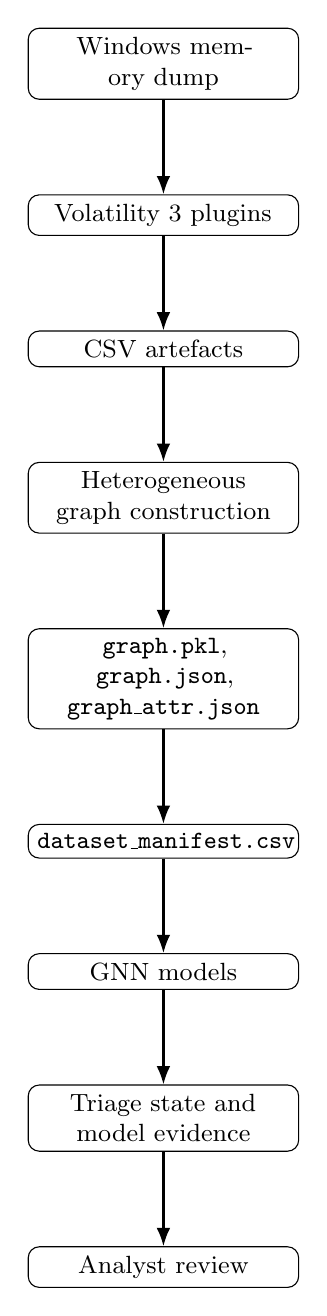
\begin{tikzpicture}[
  node distance=1.2cm,
  every node/.style={draw, rounded corners, align=center, font=\small, text width=3.2cm},
  arrow/.style={-{Latex}, thick}
]
\node (memoryDump) {Windows memory dump};
\node (vol3) [below=of memoryDump] {Volatility 3 plugins};
\node (csvFiles) [below=of vol3] {CSV artefacts};
\node (graphBuild) [below=of csvFiles] {Heterogeneous graph construction};
\node (graphFiles) [below=of graphBuild] {\texttt{graph.pkl}, \texttt{graph.json}, \texttt{graph\_attr.json}};
\node (manifest) [below=of graphFiles] {\texttt{dataset\_manifest.csv}};
\node (gnnModels) [below=of manifest] {GNN models};
\node (evidence) [below=of gnnModels] {Triage state and model evidence};
\node (analyst) [below=of evidence] {Analyst review};
\draw[arrow] (memoryDump) -- (vol3);
\draw[arrow] (vol3) -- (csvFiles);
\draw[arrow] (csvFiles) -- (graphBuild);
\draw[arrow] (graphBuild) -- (graphFiles);
\draw[arrow] (graphFiles) -- (manifest);
\draw[arrow] (manifest) -- (gnnModels);
\draw[arrow] (gnnModels) -- (evidence);
\draw[arrow] (evidence) -- (analyst);
\end{tikzpicture}
\caption{End-to-end memory-forensics and graph-learning pipeline.}
\label{fig:pipeline}
\end{figure}

\section{Extraction Layer}

The extraction layer runs Volatility 3 plugins and saves outputs in each sample folder \cite{volatility3docs}. This design makes the pipeline repeatable. It also separates raw forensic extraction from machine learning. This is useful because the same CSV artefacts can be used for manual review, rule-based scoring, and model training.

The extraction layer is intentionally conservative. It prefers stable plugin outputs over experimental plugins that may change between Volatility versions. When a plugin file is missing for a sample, downstream stages record a pipeline health flag instead of failing silently.

\section{Graph Layer}

The graph layer builds a heterogeneous system graph. The graph is stored as \texttt{graph.pkl} for Python processing and \texttt{graph.json} for inspection or dashboard use. The graph structure is important because it keeps relationships between entities. For example, a memory region can be connected to the process it belongs to, and a network connection can be connected to the process that owns it.

The graph also includes behaviour-intent edges. These edges do not only show basic ownership. They add security meaning, such as injection intent, C2 intent, credential-access intent, persistence behaviour, or suspicious parent-child relations, which correspond to well-documented adversary techniques \cite{mitre2026enterprise}, \cite{mitre2026t1055}, \cite{mitre2026t1486}. This improves the model input because it gives both structure and security context.

\section{Triage and Graph Attributes}

The rule-based triage layer creates \texttt{filtered\_malicious.json} and \texttt{graph\_attr.json}. These files contain structured signals such as suspicious PIDs, maximum process score, attack steps, injection counts, C2-style connections, and label signals. These attributes are not used to replace deep learning. They are used to support feature engineering and analyst explanation.

This hybrid design is practical. Rules are transparent and easy to inspect. GNN models can learn structural patterns that rules may miss. The final analysis can use both.

\section{Dataset Manifest Design}

The dataset manifest is the central dataset file. It links each graph folder to its label, family, graph counts, verdict fields, graph attributes, uncertainty status, governance fields, and pipeline health flags. The repository maintains manifests under both \texttt{extracted\_data} and \texttt{extracted\_csvs}; they share the same artefact contracts but differ in row count and labelling governance (Chapter~\ref{ch:methodology}, Table~\ref{tab:dual_corpus}). This supports reproducibility because a model run can be traced back to the exact folders and artefacts used \cite{goodman2016reproducibility}.

The manifest also records whether graph creation, filtering, and analysis were successful. This prevents silent failures from being treated as valid training data. Table~\ref{tab:artefact_contracts} summarises key artefact contracts used across the pipeline.

\begin{table}[htbp]
\centering
\caption{Core artefact files and their role in the pipeline.}
\label{tab:artefact_contracts}
\footnotesize
\setlength{\tabcolsep}{4pt}
\renewcommand{\arraystretch}{1.25}
\begin{tabularx}{\textwidth}{@{}>{\raggedright\arraybackslash}p{0.30\textwidth} >{\raggedright\arraybackslash}p{0.24\textwidth} >{\raggedright\arraybackslash}X@{}}
\toprule
\textbf{File} & \textbf{Producer} & \textbf{Purpose} \\
\midrule
\texttt{graph.pkl} & \texttt{build\_graph.py} & Canonical graph object for machine learning and analysis \\
\texttt{filtered\_malicious.json} & \texttt{filter\_malicious.py} & Triage evidence and suspicious process identifier list \\
\texttt{graph\_attr.json} & \texttt{build\_graph.py} & Graph-level attributes and label signals \\
\texttt{analysis\_report.json} & \texttt{analyze\_graph.py} & Per-sample graph summary and attack chain \\
\texttt{dataset\_manifest.csv} & \texttt{build\_dataset.py} & Dataset index for training and evaluation \\
\bottomrule
\end{tabularx}
\end{table}

\section{Model Stack}

The model stack has three main paths:

\begin{itemize}
\item \textbf{Binary GNN baseline:} predicts malware probability and supports calibrated thresholding.
\item \textbf{Malware one-class model:} scores how close a sample is to learned malware behaviour.
\item \textbf{Benign one-class model:} scores how close a sample is to learned benign behaviour.
\end{itemize}

Figure~\ref{fig:two_model} shows how the two-model path combines conformity scores with heuristic risk to produce triage states.

\begin{figure}[htbp]
\centering
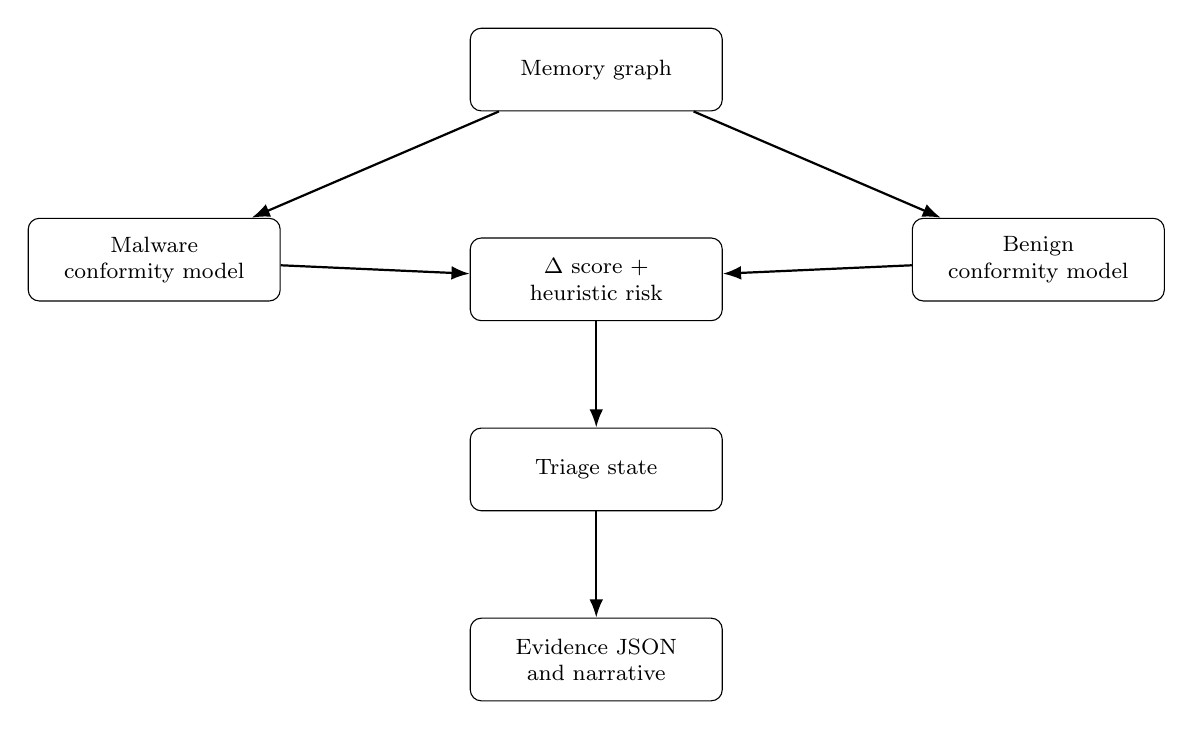
\begin{tikzpicture}[
  node distance=1.35cm and 2.2cm,
  flowbox/.style={draw, rounded corners, align=center, font=\footnotesize,
    minimum width=3.2cm, minimum height=1.05cm, inner sep=4pt},
  arrow/.style={-{Latex}, thick}
]
\node (g) [flowbox] {Memory graph};
\node (m) [flowbox, below left=1.35cm and 2.4cm of g] {Malware\\conformity model};
\node (b) [flowbox, below right=1.35cm and 2.4cm of g] {Benign\\conformity model};
\node (d) [flowbox, below=1.6cm of g] {$\Delta$ score +\\heuristic risk};
\node (t) [flowbox, below=of d] {Triage state};
\node (e) [flowbox, below=of t] {Evidence JSON\\and narrative};
\draw[arrow] (g) -- (m);
\draw[arrow] (g) -- (b);
\draw[arrow] (m) -- (d);
\draw[arrow] (b) -- (d);
\draw[arrow] (d) -- (t);
\draw[arrow] (t) -- (e);
\end{tikzpicture}
\caption{Two-model analysis flow from graph to structured evidence.}
\label{fig:two_model}
\end{figure}

The two-model analysis combines malware conformity and benign conformity, drawing on one-class deep learning principles \cite{ruff2018deep}, \cite{pang2021deep}. This is useful because a memory snapshot can be suspicious but not clearly known malware. The output states include likely malicious, likely benign, anomalous unknown, and needs analyst review.

\section{Evidence Design}

The project is designed to preserve evidence. Analysis outputs include top graph attributes, top nodes, edge pairs, reasoning types, confidence fields, and a short narrative. This makes the result more useful for incident response, consistent with the argument that interpretability must be treated as a core requirement \cite{doshi2017interpretable}. Explanation methods such as GNNExplainer \cite{ying2019gnnexplainer} provide a direction for future work. An analyst can start from the model output and then check the related graph artefacts or raw CSV rows.

\section{Interface Between Triage Rules and Learning}

The triage layer and the GNN layer are connected but not identical. Triage rules operate on interpretable thresholds and pattern checks. GNNs operate on learned combinations of structure and attributes. The system design allows three interaction modes:

\begin{enumerate}
\item \textbf{Rules only:} analysts rely on verdicts and JSON evidence without model scores.
\item \textbf{Rules + binary model:} analysts use probability and calibrated states with evidence.
\item \textbf{Rules + two-model scores:} analysts compare malware and benign conformity to detect ambiguity.
\end{enumerate}

This flexibility supports different organisational maturity levels. A lab may use rules only while collecting more data. A research team may enable GNN paths when checkpoints and manifests are stable.

\section{Final Redesign Additions}

The final implementation adds several controls around the original model stack. These additions do not change the basic memory-dump to graph pipeline. They make the pipeline more explicit about label quality, uncertainty, and feature leakage.

First, the manifest now supports governance fields such as \texttt{benign\_subtype}, \texttt{label\_quality\_flag}, \texttt{label\_quality\_reason}, and \texttt{train\_eligible}. These fields separate clean benign data from ambiguous \texttt{NoVirus} controls. This distinction is important because a benign folder name is not the same as a clean enterprise baseline.

Second, the training path can mask graph attributes that come directly from rule-based triage. The \texttt{no\_manifest\_leakage} profile keeps structural and graph-derived signals while suppressing manifest features such as maximum score, attack steps, injection counts, and C2 counts. This enables a fairer test of whether graph structure adds information beyond the triage layer.

Third, the analysis path includes calibrated abstention modes. The legacy design could route all samples to analyst review when binary and dual one-class scores disagreed. The revised design keeps the safe analyst-review state but records the reason for abstention, supports threshold calibration, and allows gate-ablation experiments.

Fourth, the graph loader can use an attack-centred subgraph view. This view extracts neighbourhoods around injection, credential-access, C2, persistence, LOLBin, and parent-child anomaly seeds. It is intended as an evaluation option for reducing memory-region and DLL hub dominance, not as a replacement for the full forensic graph.

Finally, conformal-routing hooks and diagnosis scripts were added for dissertation evaluation. These support reproducible measurement of review routing, decisive coverage, and uncertainty geometry. They should be read as research instrumentation rather than a claim of production EDR readiness.

\section{Dashboard and Operational Integration}

The repository also contains server and dashboard components. The API supports memory dump upload, plugin execution, graph pipeline execution, and model scanning \cite{fastapi2026docs}. The dashboard client can request a model scan for a dump session when \texttt{graph.pkl} exists. This shows a possible operational route for the research: memory dump upload, Volatility extraction, graph build, model scan, and analyst review in a user interface.

The operational path is optional for dissertation evaluation. The core research evidence comes from the batch pipeline and manifest, not from live UI demos.

\section{Design Rationale by Layer}

\subsection{Why separate extraction and learning}

Extraction and learning are separated so that forensic outputs remain valid even when model code changes. If a GNN architecture is replaced, the underlying CSV and graph artefacts should still be usable for manual review. This separation also helps debugging: when a score is unexpected, analysts can inspect triage JSON and plugin outputs without retraining models.

\subsection{Why use both rules and GNNs}

Rules encode transparent heuristics that security teams already understand. GNNs can combine many weak signals across structure. The hybrid design avoids two extremes: pure rules that miss complex patterns, and pure deep learning that behaves like a black box. Graph attributes from rules are included as features, so the model can learn when to trust or discount heuristic signals.

\subsection{Why graph-level classification}

Node-level classification would require node labels that are expensive to produce in memory forensics. Graph-level labels (malware vs benign for the snapshot) match the folder-level supervision available in this corpus. Graph-level outputs also match operational questions such as ``should this memory image be prioritised for deeper review?''

\section{Failure Handling and Health Flags}

The manifest records \texttt{filter\_ok}, \texttt{graph\_ok}, and \texttt{analyze\_ok}. If any step fails, the row should not enter training silently. This design follows good MLOps practice for research code \cite{sculley2015debt}.

Common failure modes include missing plugin CSV files, empty process lists, graph build exceptions, and analysis timeouts on very large graphs. Health flags make these cases visible in evaluation tables and help explain unexpected metric changes between manifest versions.

\section{Security and Privacy Considerations in Design}

Memory dumps may contain passwords, personal documents, browser history, and other sensitive data. The system design therefore assumes secure storage, restricted access, and controlled sharing. The dashboard/API path should run only in trusted lab environments.

For dissertation reporting, aggregated statistics and anonymised examples are preferred over raw command lines or host-identifying strings. This reduces ethical risk while still allowing technical discussion of malware behaviour.

\chapter{Implementation}
\label{ch:implementation}

\section{Development Environment}

The project is implemented mainly in Python. It uses Volatility 3 for forensic extraction \cite{volatility3docs}, pandas for CSV processing \cite{mckinney2010pandas}, NetworkX for graph construction \cite{hagberg2008networkx}, PyTorch and PyTorch Geometric for deep learning \cite{paszke2019pytorch}, \cite{fey2019pyg}, and FastAPI for the backend service \cite{fastapi2026docs}. The dashboard side uses TypeScript and web API routes to interact with the model scan flow.

The implementation follows a script-oriented research codebase. Each major step has a command-line entry point. This makes it easier to rerun one stage after fixing a bug without rebuilding the entire corpus.

\section{Main Repository Components}

The main implementation components are:

\begin{itemize}
\item \texttt{auto\_vol.py}: runs Volatility extraction over memory dumps.
\item \texttt{build\_graph.py}: builds heterogeneous graphs from CSV artefacts.
\item \texttt{filter\_malicious.py}: produces triage signals and suspicious evidence.
\item \texttt{analyze\_graph.py}: creates graph-level analysis reports.
\item \texttt{build\_dataset.py}: builds the dataset manifest.
\item \texttt{dataset.py}: loads graphs into PyTorch Geometric format.
\item \texttt{model.py}: defines GIN, GraphSAGE, GAT, and GINE classifiers.
\item \texttt{one\_class\_gnn.py}: defines one-class GINE utilities.
\item \texttt{train\_binary\_model.py}: trains the binary GNN baseline.
\item \texttt{train\_malware\_model.py} and \texttt{train\_benign\_model.py}: train one-class models.
\item \texttt{analyze\_binary\_model.py}: produces calibrated binary model analysis.
\item \texttt{analyze\_two\_model.py}: combines malware and benign model outputs.
\item \texttt{model\_scan.py}: runs model scanning for one upload-session graph.
\item \texttt{server.py}: exposes the extraction, graph, IOC, and scan workflow through an API.
\end{itemize}

\subsection{Extraction and graph build}

\texttt{auto\_vol.py} orchestrates plugin execution and writes \texttt{windows\_*.csv} files into each sample directory. \texttt{build\_graph.py} reads these tables, normalises identifiers, and creates nodes and edges. The script also writes \texttt{graph.pkl} and \texttt{graph.json}. The JSON form supports manual inspection and dashboard rendering.

\texttt{filter\_malicious.py} runs after an initial graph exists. It identifies suspicious PIDs and writes triage metadata used later as graph attributes. This step connects rule-based forensic reasoning with machine-learning features.

\subsection{Dataset and model code}

\texttt{build\_dataset.py} walks the corpus and writes \texttt{dataset\_manifest.csv}. The manifest is the single index used by training and evaluation scripts. \texttt{dataset.py} converts each graph into a PyTorch Geometric \texttt{Data} object with consistent feature shapes.

\texttt{model.py} defines the GNN backbones and graph-level classifier head. The implementation uses global pooling and concatenates graph attributes before the final layer. \texttt{one\_class\_gnn.py} provides encoders and scoring utilities for the malware and benign conformity models.

\section{Data Contracts}

The project uses clear file contracts. Each sample can produce:

\begin{itemize}
\item \texttt{windows\_*.csv} plugin outputs,
\item \texttt{graph.pkl},
\item \texttt{graph.json},
\item \texttt{filtered\_malicious.json},
\item \texttt{graph\_attr.json},
\item \texttt{analysis\_report.json}.
\end{itemize}

At dataset level, the main output is \texttt{dataset\_manifest.csv}. This file is used by the dataset loader and training scripts. Keeping these files consistent is important because machine learning results depend on stable input shape and meaning.

If a contract changes, the project expects coordinated updates in the loader, manifest builder, and analysis scripts. Hidden schema drift is a common source of technical debt in ML systems \cite{sculley2015debt}.

\section{Node and Edge Implementation}

The graph schema is based on real memory-forensics entities. Processes, threads, DLLs, memory regions, network connections, handles, drivers, and kernel objects become nodes. Relationships become typed edges. The graph therefore represents a system snapshot as a connected behaviour structure.

This approach is stronger than a simple count table because it preserves relationships. For example, the model can learn that injected memory connected to a process with unusual network activity may be more important than an isolated count of memory regions.

Edge typing also allows the GINE encoder to treat different relations differently. This is useful when injection edges and ownership edges carry different security meaning.

\section{Why GINE and What Alternatives Were Considered}

\subsection{Why GINE over untyped convolutions}

Forensic graphs are heterogeneous: edge types encode distinct semantics (parent--child, DLL load, injection, network ownership, behaviour-intent links). Standard GCN or mean-aggregation layers treat all edges similarly and can blur type-specific signals. GINE extends GIN with edge-conditioned message functions so each relation type contributes separately \cite{xu2019gin}. That matches the design goal: preserve forensic meaning in the message-passing path rather than collapsing relations into unlabeled adjacency.

\subsection{Why graph-level classification, not node labels}

Memory dumps in this corpus provide snapshot-level supervision (\texttt{WithVirus} vs \texttt{NoVirus}). Node-level malware labels are not available without expensive manual annotation. Graph-level classification answers the operational question ``should this memory image be prioritised?'' and aligns with manifest labels, at the cost of ignoring which specific process caused the label.

\subsection{Supported backbones and expected trade-offs}

\texttt{model.py} implements GIN, GraphSAGE, GAT, and GINE with the same pooling head and graph-attribute concatenation. Table~\ref{tab:gnn_comparison} (generated by \texttt{scripts/generate\_eval\_latex.py} after grouped CV) is the intended comparison point. Until CV JSON files exist, cells remain placeholders.

\begin{itemize}
\item \textbf{GIN:} strong baseline for graph classification; no edge-type conditioning.
\item \textbf{GraphSAGE:} inductive neighbourhood sampling; useful if graphs grow beyond current corpus scale.
\item \textbf{GAT:} attention over neighbours; higher compute on large graphs (many memory-region nodes).
\item \textbf{GINE:} default for binary and one-class paths because edge types are informative.
\end{itemize}

\subsection{What did not work well in practice}

Three trade-offs appeared during development. \textbf{Small $n$:} with 30 graphs, validation folds are unstable; family grouping is necessary but reduces effective training size per fold. \textbf{Train time vs graph size:} samples above 20,000 nodes dominate batch memory; training epochs are costly relative to tabular baselines on manifest features alone. \textbf{Heuristic features vs pure learning:} graph attributes already encode strong triage signals; GNN gains may be modest unless structure adds information beyond \texttt{graph\_attr.json}---an open question for the tabular-vs-GNN comparison in Chapter~\ref{ch:evaluation}.

\section{GNN Implementation}

The GNN models perform message passing over the graph \cite{hamilton2020graph}. Each graph is converted into PyTorch Geometric data \cite{fey2019pyg} with:

\begin{itemize}
\item \texttt{x} for node features,
\item \texttt{edge\_index} for graph connectivity,
\item \texttt{edge\_attr} for edge-type IDs,
\item \texttt{graph\_attr} for graph-level features,
\item \texttt{batch} for mini-batch processing.
\end{itemize}

The model then creates a graph-level representation using pooling operations. The implementation uses mean, max, and sum pooling. The pooled graph vector is joined with graph-level attributes before final classification or scoring.

\subsection{Training configuration}

The binary trainer supports class-weight tuning, early stopping, and optional learning-rate scheduling. Default training uses multiple epochs with validation-based model selection. The script can sweep positive-class weights to balance recall and specificity on small validation folds.

One-class trainers learn embedding-space boundaries for malware-only or benign-only subsets. These models are later used by \texttt{analyze\_two\_model.py} to compare conformity scores on new graphs.

\section{Evidence and Inference Implementation}

The analysis scripts do more than return a score. They enrich nodes and edges with evidence metadata, align features with checkpoint expectations, apply calibration where needed, compute uncertainty fields, and write structured JSON so analysts can audit outputs.

The two-model analysis produces fields such as:

\begin{itemize}
\item malware pattern score,
\item benign conformity score,
\item delta score,
\item triage state,
\item reasoning types,
\item behavioural findings,
\item model evidence,
\item narrative explanation.
\end{itemize}

\texttt{model\_scan.py} exposes a single-graph inference path for the API workflow. This is useful for upload-session analysis in the dashboard prototype.

\section{Implementation Challenges}

Three challenges appeared repeatedly during development.

\textbf{Missing or partial plugin output.} Not every sample had identical CSV coverage. The graph builder had to tolerate absent files while still recording health flags in the manifest.

\textbf{Graph-size variation.} The corpus includes graphs from 86 nodes to more than 27,000 nodes. Batch training therefore required careful memory use and padding strategies.

\textbf{Noisy benign labels.} Many NoVirus folders produced HIGH or CRITICAL rule-based verdicts. The implementation response was to add \texttt{uncertain} flags and analyst-review states instead of forcing clean benign labels.

\section{Reproducibility}

Reproducibility is supported by the manifest, saved model metadata, stable graph attributes, and fixed file contracts \cite{goodman2016reproducibility}. A future reader can inspect which samples were used, which graph attributes were present, and which steps completed successfully. This is important in cybersecurity research because small implementation changes can alter results, a problem known as hidden technical debt in machine learning systems \cite{sculley2015debt}.

Appendix~\ref{app:repro} lists recommended commands to rebuild the dataset and regenerate dissertation figures.

\section{Per-Module Implementation Notes}

\subsection{\texttt{build\_graph.py}}

The graph builder reads plugin CSV files and maps rows to node dictionaries. Processes are linked with parent-child relations when \texttt{pstree} or equivalent information is available. DLL and memory-region nodes attach to process nodes with typed edges. Network connections link to owning processes and remote IP nodes.

The builder also computes derived indicators such as suspicious process scores and attack-step counts used later in triage. When enrichment is enabled, behaviour-intent edges are added from rule outcomes rather than from raw plugin rows alone.

\subsection{\texttt{filter\_malicious.py}}

The filter stage identifies suspicious PIDs and writes \texttt{filtered\_malicious.json}. This file includes metadata used by both graph attribute generation and analyst review. The filter is intentionally readable: an analyst can open the JSON file and see which PIDs triggered suspicion without reading model code.

\subsection{\texttt{analyze\_graph.py}}

The analysis stage produces \texttt{analysis\_report.json} with graph summaries, attack-chain steps, and structured suspicious-node listings. Version 3 of the analyser enriches outputs used by the dissertation case studies. The WannaCry example in Chapter~\ref{ch:evaluation} comes directly from this file format.

\subsection{\texttt{dataset.py} and training scripts}

The dataset loader reads \texttt{dataset\_manifest.csv}, loads each \texttt{graph.pkl}, and converts graphs to PyTorch Geometric batches. Feature alignment checks help prevent silent mismatches between training and inference checkpoints.

\texttt{train\_binary\_model.py} trains the supervised baseline. \texttt{train\_malware\_model.py} and \texttt{train\_benign\_model.py} train one-class encoders. \texttt{analyze\_binary\_model.py} and \texttt{analyze\_two\_model.py} generate JSON outputs for single samples or batches.

\subsection{\texttt{server.py} and \texttt{model\_scan.py}}

The server exposes endpoints for extraction, graph build, and scanning workflows. \texttt{model\_scan.py} supports session-based inference when a graph already exists for an uploaded dump. This path is useful for interactive demos but is not required for batch evaluation on the 30-sample corpus.

\section{Hyperparameters and Training Defaults}

Table~\ref{tab:hyperparams} summarises main training defaults used in the binary trainer. These values are implementation defaults rather than fully tuned optimal settings. They are reported here for reproducibility.

\begin{table}[htbp]
\centering
\caption{Representative binary training defaults (\texttt{train\_binary\_model.py}).}
\label{tab:hyperparams}
\begin{tabular}{ll}
\toprule
\textbf{Setting} & \textbf{Typical value / behaviour} \\
\midrule
Epochs & Configurable (default in script) \\
Optimiser & Adam-style update with weight decay \\
Learning rate schedule & Cosine annealing supported \\
Early stopping & Enabled on validation F1 stall \\
Class weight & Auto or manual positive-class weight \\
Validation split & Hold-out split from manifest rows \\
Output & Checkpoint and metadata JSON \\
\bottomrule
\end{tabular}
\end{table}

One-class trainers follow a similar pattern but optimise embedding-space objectives rather than binary cross-entropy. Analysis scripts load checkpoints and align feature dimensions before inference. When checkpoint files are absent, analysis scripts cannot produce model scores and the evaluation must rely on triage artefacts alone.

\section{Performance and Resource Considerations}

Large graphs dominate memory use. Samples with more than 20,000 nodes require efficient batching and may limit hyperparameter search. The project mitigates this by graph-level classification (one label per graph) rather than node-level classification across the full corpus.

CPU preprocessing time is also significant. Volatility extraction and graph construction can take much longer than one training epoch on small data. For research planning, artefact generation should be treated as a first-class timeline item, not as a one-time preliminary step.

\section{Testing and Validation During Development}

During development, samples were inspected manually at three checkpoints: after CSV extraction, after graph build, and after analysis JSON generation. This manual review caught issues such as missing plugin files, unexpected empty graphs, and extreme node counts. Manual review is not scalable to thousands of hosts, but it was valuable for a 30-sample research corpus.

Regression checks should include: (1) manifest row count stable, (2) no missing health flags, (3) graph node counts within expected order of magnitude for family, and (4) analysis verdicts present. The dissertation figures provide a quick visual regression check for corpus-level shifts when graph rules change.

\chapter{Evaluation and Discussion}
\label{ch:evaluation}

\section{Central Empirical Finding}

The strongest result from the current corpus is not a detection F1 score. It is the systematic mismatch between benign folder labels and rule-based triage signals.

In \texttt{dataset\_manifest.csv} ($n{=}30$), \textbf{14 of 15} benign-labelled (\texttt{NoVirus}) rows are marked \texttt{uncertain=True}. Reasons include HIGH or CRITICAL verdicts, elevated process scores, injection counts, and C2-style connection counts despite benign labels. Only the W32.MyDoom.A.-NoVirus row is not uncertain. Malware-labelled rows are not flagged uncertain in the manifest.

Figure~\ref{fig:uncertainty_benign} summarises the split. Figure~\ref{fig:dataset_overview} places it in the wider label balance. This pattern means folder naming is an imperfect proxy for ground truth: ``clean'' baselines in memory forensics can still contain suspicious artefacts from security tools, prior activity, or capture timing.

\begin{figure}[htbp]
\centering
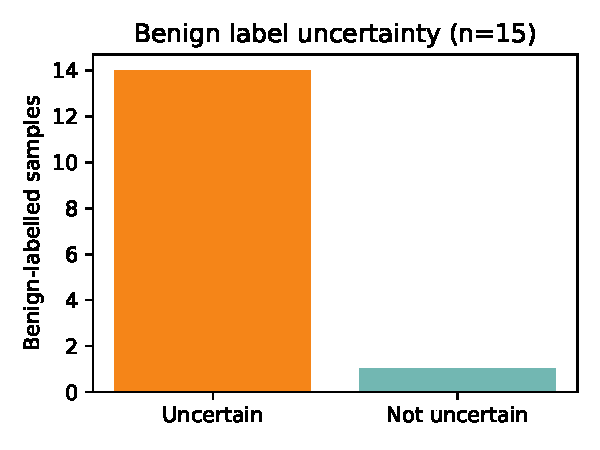
\includegraphics[width=0.62\textwidth]{fig_uncertainty_benign.pdf}
\caption{Benign-labelled samples: uncertain vs not uncertain ($n{=}15$).}
\label{fig:uncertainty_benign}
\end{figure}

For machine learning, uncertain benign rows should be excluded, down-weighted, or reported separately in evaluation. Treating all NoVirus folders as definitively benign will inflate false conclusions about separability.

\section{Proof-of-Concept Scope}

This chapter evaluates whether the pipeline produces consistent artefacts, meaningful graphs, and auditable evidence on a small research corpus. It does \textbf{not} claim production malware detection performance. Quantitative ML tables use placeholders until grouped cross-validation is run and checkpoints are archived (see \S\ref{sec:quant_ml_eval}).

\section{Descriptive Corpus Statistics}

Table~\ref{tab:corpus_summary} summarises manifest-level scale statistics (from \texttt{figures/dataset\_stats.json}). Graph size spans more than two orders of magnitude; both labels include very large graphs.

\begin{table}[htbp]
\centering
\caption{Corpus summary statistics (30 manifest rows).}
\label{tab:corpus_summary}
\begin{tabular}{lrrrr}
\toprule
\textbf{Statistic} & \textbf{Min} & \textbf{Median} & \textbf{Max} & \textbf{Notes} \\
\midrule
Nodes (all) & 86 & 18,036 & 27,362 & MyDoom pair smallest \\
Edges (all) & 7 & 21,544 & 32,556 & \\
Malware-labelled & 15 & --- & --- & No uncertain flags \\
Benign-labelled & 15 & --- & --- & 14 uncertain \\
\bottomrule
\end{tabular}
\end{table}

\begin{figure}[htbp]
\centering
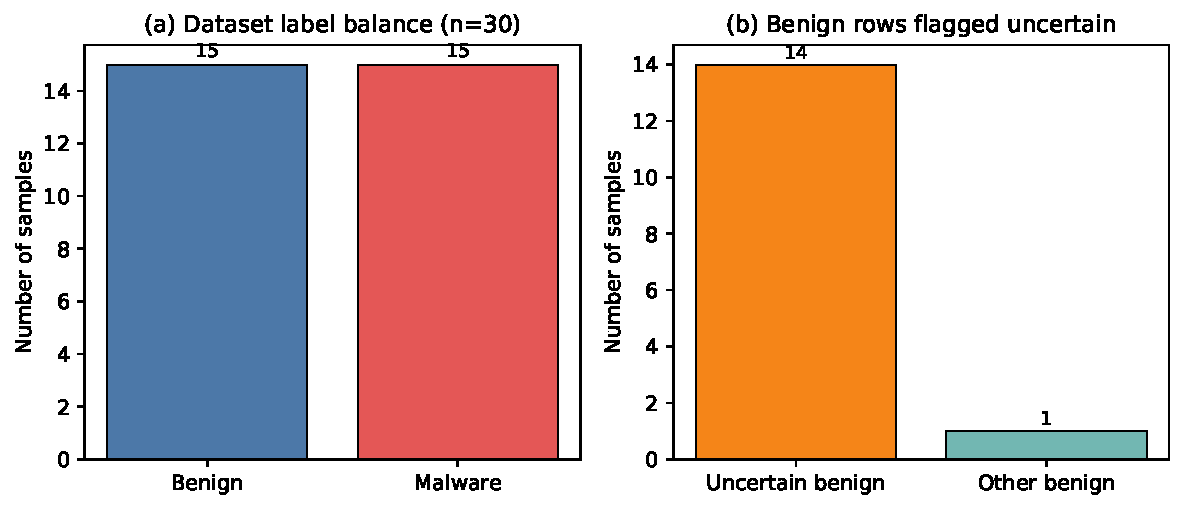
\includegraphics[width=0.95\textwidth]{fig_dataset_overview.pdf}
\caption{Dataset composition: malware vs benign labels and uncertain benign subset.}
\label{fig:dataset_overview}
\end{figure}

\begin{figure}[htbp]
\centering
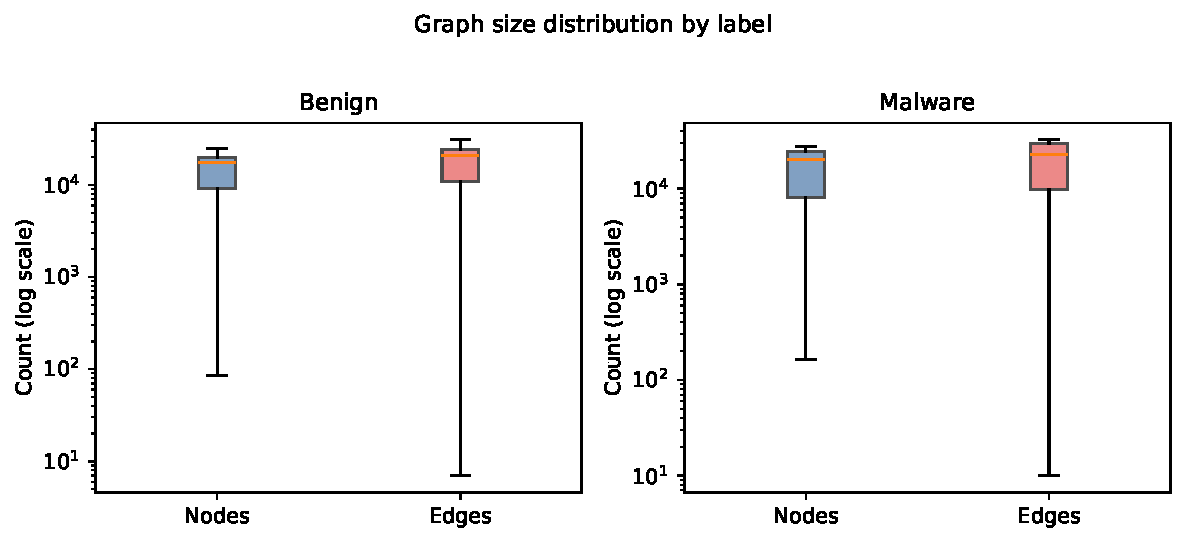
\includegraphics[width=0.95\textwidth]{fig_graph_scale.pdf}
\caption{Node and edge counts by label (log scale).}
\label{fig:graph_scale}
\end{figure}

All listed rows completed filter, graph, and analysis stages (\texttt{filter\_ok}, \texttt{graph\_ok}, \texttt{analyze\_ok}), giving a stable artefact base for discussion.

\section{Rule-Based Triage Analysis}

Rule-based signals in the manifest show false-positive pressure on NoVirus rows. Figure~\ref{fig:forensic_signals} compares mean injection count, C2 connections, and maximum process score by label. Malware-labelled means are not uniformly higher than benign-labelled means for every signal.

\begin{figure}[htbp]
\centering
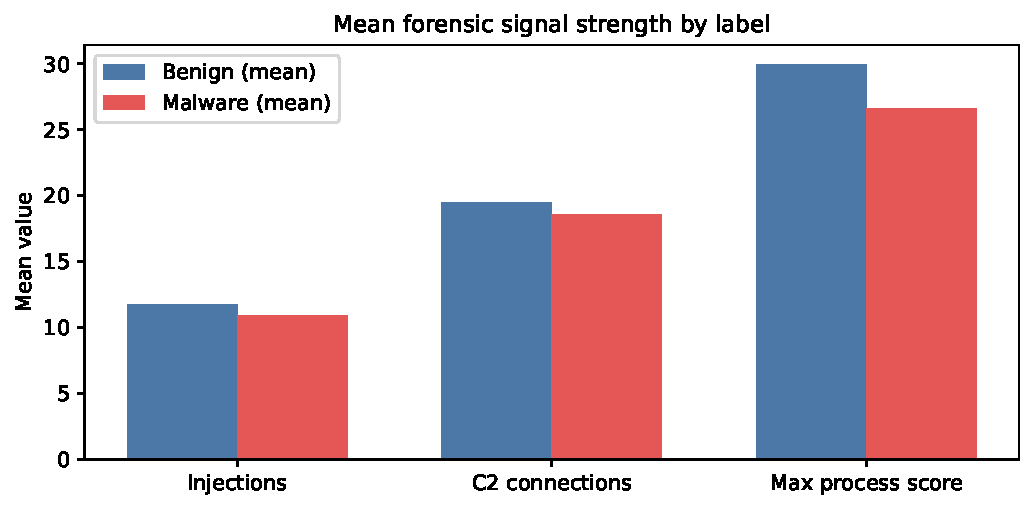
\includegraphics[width=0.85\textwidth]{fig_forensic_signals.pdf}
\caption{Mean forensic signal values by label (manifest-derived).}
\label{fig:forensic_signals}
\end{figure}

Figure~\ref{fig:verdict_dist} shows that most samples receive HIGH or CRITICAL verdicts. Only the MyDoom pair reports LOW verdicts. Benign-labelled rows therefore often receive the same verdict bands as malware-labelled rows, which explains the uncertain flags.

\begin{figure}[htbp]
\centering
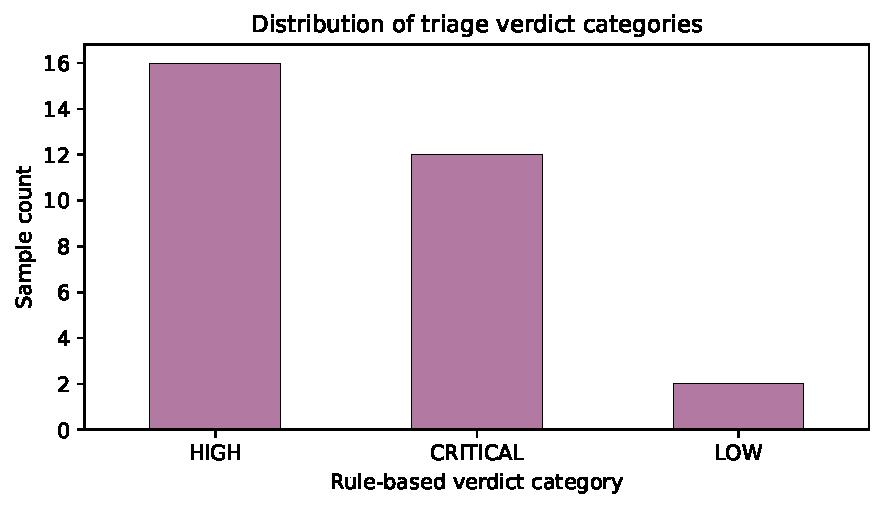
\includegraphics[width=0.78\textwidth]{fig_verdict_distribution.pdf}
\caption{Rule-based triage verdict categories across the corpus.}
\label{fig:verdict_dist}
\end{figure}

Figure~\ref{fig:family_coverage} shows each malware family contributes paired WithVirus and NoVirus rows. Family-grouped splits are mandatory for honest evaluation \cite{sommer2010outside}.

\begin{figure}[htbp]
\centering
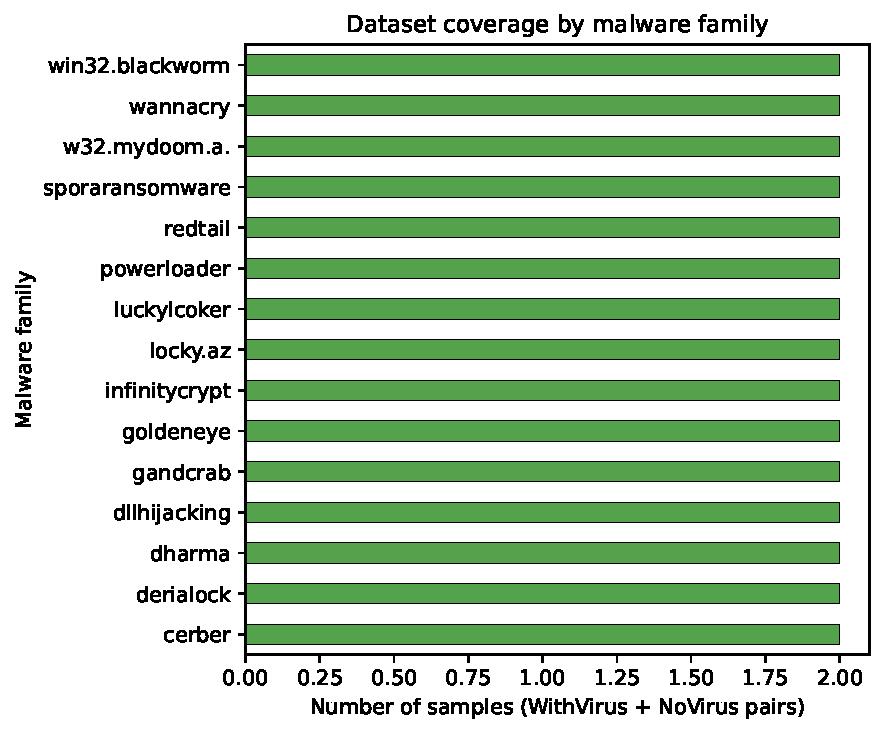
\includegraphics[width=0.72\textwidth]{fig_family_coverage.pdf}
\caption{Manifest rows per malware family.}
\label{fig:family_coverage}
\end{figure}

\section{Quantitative Machine Learning Evaluation}
\label{sec:quant_ml_eval}

Grouped evaluation is implemented in \texttt{train.py} (StratifiedGroupKFold by \texttt{family}), \texttt{train\_binary\_model.py}, and \texttt{scripts/tabular\_baselines.py}. Saved \texttt{results\_*.json} files were not present in the repository at writing time; Table~\ref{tab:gnn_comparison}--\ref{tab:cv_protocol} therefore show ``--'' placeholders. After running experiments, regenerate tables with:

\begin{verbatim}
python train.py extracted_data/dataset_manifest.csv --cv stratified_group \
  --group-by family --model gine --epochs 80 --seed 42
python scripts/tabular_baselines.py
python scripts/generate_eval_latex.py
\end{verbatim}

% Auto-generated by scripts/generate_eval_latex.py
% Tabular baselines only; Track 1 GNN CV not reported numerically.

\subsection{Tabular baselines (manifest graph-level features)}
\begin{table}[htbp]
\centering
\caption{Tabular baseline CV on \texttt{extracted\_data} manifest (\texttt{tabular\_baselines.py}). Reference only---primary ML results are Tracks 2/3.}
\label{tab:tabular_baselines}
\begin{tabular}{lcccc}
\toprule
\textbf{Model} & \textbf{Precision} & \textbf{Recall} & \textbf{F1} & \textbf{ROC-AUC} \\
\midrule
Logistic Regression & 0.500 & 0.467 & 0.469 & 0.489 \\
Random Forest & 0.687 & 0.667 & 0.631 & 0.711 \\
\bottomrule
\end{tabular}
\end{table}


\subsection{Evaluation figures (placeholders until predictions exist)}

When \texttt{outputs/predictions.csv} is produced from grouped CV, \texttt{scripts/generate\_eval\_latex.py} can render confusion-matrix and ROC PDFs (\texttt{fig\_confusion\_matrix.pdf}, \texttt{fig\_roc\_curve.pdf}). Until then, only manifest-derived figures (including Figure~\ref{fig:uncertainty_benign}) are included.

% Uncomment after running generate_eval_latex.py with predictions:
% \begin{figure}[htbp]
% \centering
% \includegraphics[width=0.55\textwidth]{fig_confusion_matrix.pdf}
% \caption{Confusion matrix for GINE (grouped CV).}
% \label{fig:confusion_matrix}
% \end{figure}
%
% \begin{figure}[htbp]
% \centering
% \includegraphics[width=0.55\textwidth]{fig_roc_curve.pdf}
% \caption{ROC curve for GINE (grouped CV).}
% \label{fig:roc_curve}
% \end{figure}

A natural comparison is tabular classifiers on \texttt{graph\_attr} features versus full-graph GNNs on the same manifest version. If tabular models match GNNs, relational structure may add little on this small, heuristic-rich corpus; if GNNs improve under grouped CV, that supports the graph design.

\section{Failure Cases and Edge Families}

\subsection{W32.MyDoom.A. pair (very small graphs)}

W32.MyDoom.A.-NoVirus (86 nodes) and W32.MyDoom.A.-WithVirus (164 nodes) are outliers. Both report LOW verdicts and zero injections; neither benign row is uncertain. Models trained mainly on large graphs may underfit or overfit on tiny topologies---pooling and normalisation should be checked on this pair.

\subsection{Cerber pair (similar scale, divergent C2 counts)}

Cerber-WithVirus (7,904 nodes) and Cerber-NoVirus (9,382 nodes) have comparable scale. The malware row reports 24 C2 connections and \texttt{lolbin\_c2\_found=True}; the benign row reports 7 C2 connections and is uncertain. Both share HIGH verdicts and six injections in the manifest. A GNN may not separate these folders if features emphasise shared injection structure more than family-specific infection cues.

\subsection{GoldenEye pair (high injection on both rows)}

GoldenEye-WithVirus has the highest injection count (41). GoldenEye-NoVirus still reports 8 injections, 13 hidden processes, and a CRITICAL verdict. This is among the clearest uncertain-benign examples: triage treats both snapshots as highly suspicious.

\subsection{WannaCry case study}

WannaCry-WithVirus (8,098 nodes) shows injection-related attack-chain steps and ransom-note signals. WannaCry-NoVirus (7,590 nodes) reports nine injections, a HIGH verdict, and \texttt{uncertain=True}. Figure~\ref{fig:wannacry_nodes} shows memory regions dominate node types---typical for VAD-heavy graphs.

\begin{figure}[htbp]
\centering
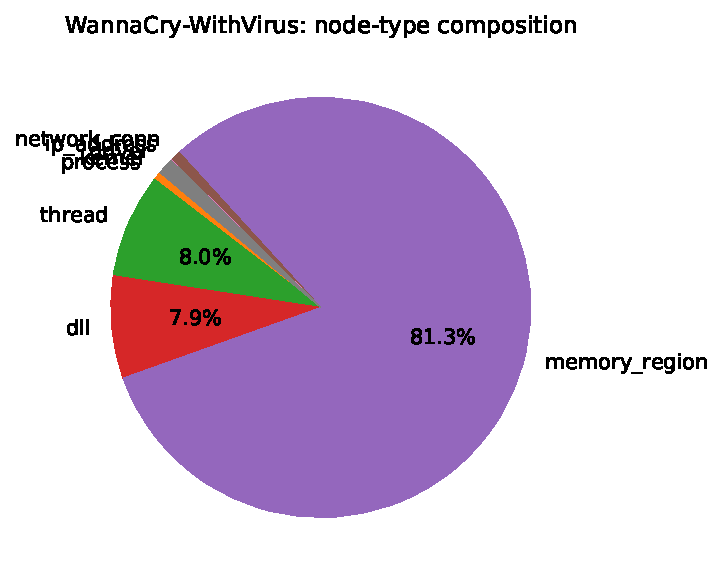
\includegraphics[width=0.62\textwidth]{fig_wannacry_node_types.pdf}
\caption{Node-type composition for WannaCry-WithVirus.}
\label{fig:wannacry_nodes}
\end{figure}

\begin{table}[htbp]
\centering
\caption{WannaCry manifest comparison (selected fields).}
\label{tab:wannacry_compare}
\begin{tabular}{lrrrr}
\toprule
\textbf{Folder} & \textbf{Label} & \textbf{Nodes} & \textbf{Injections} & \textbf{Uncertain} \\
\midrule
WannaCry-WithVirus & Malware & 8,098 & 7 & No \\
WannaCry-NoVirus & Benign & 7,590 & 9 & Yes \\
\bottomrule
\end{tabular}
\end{table}

\subsection{When a GNN may not help}

GNNs add value when relational structure carries signal beyond graph-level heuristics. They may add little when: (1) labels are dominated by triage noise; (2) graphs differ mainly in size, not infection topology; (3) train and test families are too few for stable grouped metrics; or (4) edge and node features already encode the decision rules. The uncertain-benign prevalence pushes toward analyst-review workflows and two-model conformity scores rather than hard binary automation.

\section{Binary and Two-Model Paths}

The binary GNN path supports calibrated probabilities and ambiguous states \cite{guo2017calibration}. On noisy labels, a single threshold can encode triage noise rather than infection state. The two-model path compares malware and benign conformity \cite{ruff2018deep}, surfacing cases where both scores are elevated---consistent with uncertain benign rows.

Saved checkpoints were not archived in the repository at writing time. Implementation capability is documented; grouped metrics require the user to train, save \texttt{*.pt} files, and regenerate LaTeX tables.

\section{Explainability}

The project records top graph attributes, important nodes, and edge pairs in JSON evidence. This is not a complete explanation method \cite{doshi2017interpretable}, but it exceeds a single opaque score. GNNExplainer \cite{ying2019gnnexplainer} remains future work.

\section{What Results Prove and Do Not Prove}

\textbf{Proven on current artefacts:}
\begin{itemize}
\item Volatility artefacts can be converted into typed graphs from 86 to 27,362 nodes.
\item Rule-based triage produces HIGH/CRITICAL verdicts on most benign-labelled rows (14/15 uncertain).
\item Manifest governance supports reproducible, family-aware evaluation design.
\item Evidence JSON and uncertainty fields are implementable alongside GNN scores.
\end{itemize}

\textbf{Not proven:}
\begin{itemize}
\item Superior detection accuracy versus production AV or EDR on enterprise hosts.
\item Generalisation to unseen malware families without grouped CV on larger $n$.
\item That GNN structure beats strong tabular baselines on the same manifest (pending experiments).
\item Robustness to adversarial graph manipulation \cite{apruzzese2023sok}.
\end{itemize}

\section{Limitations}

\begin{itemize}
\item Small corpus ($n{=}30$) with high metric variance under grouped CV.
\item Noisy benign labels (14/15 uncertain).
\item Family-level pairing limits independent test families.
\item Capture timing and Windows build affect plugin output.
\item Heuristic graph attributes couple rules and learning.
\item Missing archived checkpoints and prediction CSVs at submission time.
\end{itemize}

Sommer and Paxson \cite{sommer2010outside} and Sculley et al.\ \cite{sculley2015debt} apply: evaluation design and pipeline debt can dominate headline metrics.

\section{Practical Value}

The pipeline supports evidence-led triage \cite{case2017memory}: organise plugin output, surface rule verdicts, attach GNN scores as a secondary signal, and export JSON for analyst review. The uncertain-benign finding is operationally relevant---teams should expect HIGH verdicts on baseline images without treating them automatically as labelling errors.

\section{Summary}

\begin{enumerate}
\item Benign-labelled rows frequently exhibit HIGH/CRITICAL triage signals (14/15 uncertain)---the central empirical finding.
\item Graph construction scales from tiny to very large memory snapshots.
\item Rule-based triage alone cannot define benign status from folder names.
\item Grouped CV and tabular baselines are implemented; numeric ML tables await experiment runs.
\item Structured evidence improves usefulness over a single probability.
\end{enumerate}

\chapter{Conclusion and Future Work}

\section{Conclusion}

This dissertation implemented a proof-of-concept pipeline for graph-based malware triage from Windows memory forensics: Volatility~3 extraction, typed memory-snapshot graphs, graph-level features, GNN scoring (GIN, GraphSAGE, GAT, GINE), and structured evidence with uncertainty fields \cite{volatility3docs}, \cite{fey2019pyg}.

The primary empirical finding is label--signal mismatch on benign baselines: \textbf{14 of 15} benign-labelled manifest rows are marked uncertain because rule-based triage still reports HIGH or CRITICAL activity. Folder names (\texttt{NoVirus}) are an imperfect proxy for ground truth. This result should be reported openly in any memory-forensics ML study, not treated as a labelling failure to hide.

Secondary contributions are reproducible engineering artefacts: manifests, data contracts, grouped evaluation scripts, tabular baselines, and JSON evidence for analyst review. Together they show that graph-based representation can organise memory-forensics evidence at scale, while detection metrics on $n{=}30$ remain feasibility evidence until larger corpora and archived checkpoints are available.

\section{Answers to Research Questions}

\textbf{RQ1: How can memory artefacts be represented as a graph?} Volatility CSV outputs map to typed nodes and edges (processes, memory regions, DLLs, network objects, intent relations). The manifest records scale and triage metadata per sample.

\textbf{RQ2: Which entities and relationships are most useful?} Process--memory and process--network links are central; intent edges align behaviour with ATT\&CK-style patterns \cite{mitre2026enterprise}. Memory-region nodes dominate graph size in case studies such as WannaCry.

\textbf{RQ3: How can GNNs support detection with readable evidence?} Binary and two-model paths combine learned scores with graph attributes, top nodes, and JSON evidence. Uncertain benign flags motivate analyst-review states rather than forced binary decisions.

\textbf{RQ4: What limitations appear on a small corpus?} High graph-size variance, 14/15 uncertain benign rows, and family pairing require grouped splits and modest claims \cite{sommer2010outside}. Placeholder metric tables document what remains to be run experimentally.

\section{Reflection on the Research Aim}

The aim---to design and evaluate a graph-based deep learning pipeline for memory-forensics malware detection---was met at the pipeline and evidence level. Extraction, graph construction, manifests, models, and analyst-facing outputs are implemented. Full quantitative detection evaluation is partial because checkpoints and \texttt{results\_*.json} files were not archived; Chapter~\ref{ch:evaluation} states that boundary explicitly.

The work does not claim GNNs outperform all alternatives on all malware. It demonstrates feasibility, foregrounds benign-label uncertainty, and specifies the next experiments (grouped CV, tabular comparison, calibration plots).

\section{Contributions}

\begin{itemize}
\item Volatility~3 extraction workflow and artefact contracts;
\item heterogeneous memory-snapshot graph schema;
\item graph-level feature engineering linked to triage;
\item GNN and tabular evaluation scripts with family-grouped CV;
\item structured evidence and uncertainty reporting;
\item dataset manifest for reproducibility;
\item optional dashboard upload-session scanning.
\end{itemize}

\section{Future Work}

\begin{itemize}
\item Expand corpus with clean enterprise baselines and known-good capture times;
\item Run and archive grouped CV for GIN/SAGE/GAT/GINE and tabular baselines; populate Table~\ref{tab:gnn_comparison};
\item Add GNNExplainer \cite{ying2019gnnexplainer} or similar graph explanations;
\item Test on families held out entirely from training;
\item Improve label curation with analyst feedback on uncertain rows;
\item Monitor feature drift across manifest versions;
\item Compare against gradient boosting and operational EDR telemetry \cite{pedregosa2011sklearn}, \cite{ucci2019survey}.
\end{itemize}

\section{Implications for Practice}

Practitioners should treat HIGH or CRITICAL verdicts on benign-labelled baselines as expected when memory contains security tools or noisy host state. Workflow: acquire memory, run plugins, build graphs, inspect triage JSON, then use GNN scores as a secondary signal. Educators can use manifests and figures without requiring enterprise-scale labelled data.

\section{Final Statement}

Graph-based deep learning is a plausible direction for memory-forensics malware triage because system behaviour is relational. The strongest outcome of this project is a reproducible, explainable path from memory dump to evidence---with honest reporting that benign labels and triage signals often disagree. Detection metrics on the current corpus should support feasibility claims only until grouped benchmarks on larger data replace the placeholders in Chapter~\ref{ch:evaluation}.

\chapter{Reflection}

\section{Project Learning}

This project improved my understanding of both memory forensics and machine learning. At the start, the work looked like a malware detection task. During development, it became clear that data representation was the most important part. If the memory artefacts are not extracted and organised correctly, the model cannot learn useful patterns.

I also learned that dissertation scope must match the evidence. The project contains ransomware families, but the research topic is broader: graph-based malware detection from Windows memory forensics. Keeping this focus improved the clarity of the writing and the evaluation.

\section{Technical Reflection}

The most difficult technical challenge was joining many Volatility outputs into one stable graph. Each plugin gives different columns and different levels of detail. The graph builder had to handle missing files, different object types, and noisy evidence. This taught me that cybersecurity machine learning depends strongly on data engineering \cite{sculley2015debt}.

Another challenge was uncertainty. Some NoVirus samples had suspicious features and HIGH or CRITICAL verdicts. Instead of ignoring this, the project records uncertainty in the manifest. This is a more honest approach and fits real forensic work, where evidence is often mixed.

Graph-size variation was also difficult for training. A graph with fewer than 200 nodes and a graph with more than 25,000 nodes appear in the same dataset. This required careful batching and realistic expectations about model stability on small data.

\section{Research Reflection}

The project also improved my research writing. The correct dissertation topic is broader than ransomware. Rewriting the work around graph-based deep learning made the argument stronger and more accurate. It also helped separate the dataset examples from the main research contribution.

Working with IEEE-style references improved my literature discipline. Each major claim should be linked to prior work or to project artefacts. This is similar to forensic reporting, where each conclusion should be linked to evidence.

\section{Professional Reflection}

This project is relevant to digital forensics, incident response, malware analysis, and security engineering. It helped me understand how a research prototype can be designed for practical analyst use. The most valuable lesson is that detection tools should explain their evidence and limitations clearly \cite{doshi2017interpretable}, \cite{case2017memory}.

If this system were deployed in a SOC environment, I would present it as a triage assistant. Analysts would still validate important cases manually. The tool would help them prioritise which memory dumps deserve deeper review.

\section{Closing Reflection}

The project shows that good cybersecurity research needs both technical implementation and careful communication. A model is not enough by itself. The data pipeline, graph design, evidence output, uncertainty handling, and documentation all matter. This learning will be useful for future work in malware analysis and defensive security.

I would advise future students on similar projects to lock artefact contracts early, publish a manifest for every experiment, and report uncertain labels openly. These habits improve trust in the final dissertation and in the underlying code.

\section{Skills Developed}

Through this project I developed practical skills in Volatility-based artefact interpretation, graph schema design, PyTorch Geometric modelling, and technical writing for dual audiences (academic examiners and security practitioners). I also learned to use manifests and JSON evidence files as first-class research outputs, not as secondary logs.

\section{What I Would Do Differently}

If starting again, I would collect more clean benign baselines from known-good enterprise images and document acquisition timing for every dump. I would also archive trained checkpoints with manifest version IDs from the first successful training run. That would make Chapter~\ref{ch:evaluation} stronger because model metrics could be reported alongside corpus statistics.

Finally, I would add automated grouped cross-validation scripts earlier in the project. This would reduce the risk of optimistic results when related family folders leak between train and test splits.

\section{Personal Outcome}

Completing this dissertation improved my confidence in building end-to-end security research systems. I now understand that writing, implementation, and evaluation must be planned together. A strong model without manifests, contracts, and evidence outputs would not meet the needs of forensic practitioners. That lesson will guide my approach in future cyber security roles and research projects.


\appendix
\chapter{Project Artefacts and Reproducibility}
\label{app:repro}

\section{Project Artefact Map}
\begin{longtable}{p{0.28\textwidth}p{0.62\textwidth}}
\toprule
\textbf{Artefact} & \textbf{Purpose} \\
\midrule
\endhead
\texttt{windows\_*.csv} & Volatility 3 plugin output for each sample \\
\texttt{graph.pkl} & NetworkX graph used by graph processing and model loading \\
\texttt{graph.json} & JSON graph representation for inspection and UI use \\
\texttt{filtered\_malicious.json} & Rule-based triage evidence and graph attributes \\
\texttt{graph\_attr.json} & Graph-level attributes and label signals \\
\texttt{analysis\_report.json} & Per-sample graph analysis report \\
\texttt{dataset\_manifest.csv} & Dataset index used for training and evaluation \\
\texttt{*.pt} model files & Saved PyTorch model checkpoints \\
\texttt{*\_meta.json} & Model metadata and calibration information \\
\bottomrule
\end{longtable}

\section{Manifest Column Glossary}
\begin{longtable}{p{0.26\textwidth}p{0.64\textwidth}}
\toprule
\textbf{Column} & \textbf{Meaning} \\
\midrule
\endhead
\texttt{sample\_id} & Numeric identifier for each graph row \\
\texttt{folder} & Directory name for the sample \\
\texttt{label} & 0 = NoVirus (benign), 1 = WithVirus (malware) \\
\texttt{family} & Malware family tag used for grouped evaluation \\
\texttt{nodes}, \texttt{edges} & Graph size statistics \\
\texttt{max\_score} & Highest suspicious process score from triage \\
\texttt{injections}, \texttt{c2\_conns} & Counts of injection and C2-style indicators \\
\texttt{verdict} & Rule-based triage verdict string \\
\texttt{uncertain} & Flag for label or baseline uncertainty \\
\texttt{filter\_ok}, \texttt{graph\_ok}, \texttt{analyze\_ok} & Pipeline health indicators \\
\bottomrule
\end{longtable}

\section{Core Plugin Set}
The project uses the following main Volatility 3 plugins: \texttt{pslist}, \texttt{psscan}, \texttt{pstree}, \texttt{malfind}, \texttt{netscan}, \texttt{cmdline}, \texttt{dlllist}, \texttt{handles}, \texttt{threads}, \texttt{vadinfo}, \texttt{filescan}, \texttt{driverscan}, \texttt{ssdt}, and \texttt{registry.hivelist}.

\section{Reproducibility Commands}
The following commands rebuild dataset artefacts, run evaluation, and regenerate dissertation tables from the repository root:

\begin{verbatim}
python build_dataset.py
python scripts/generate_dissertation_figures.py

# Grouped CV -- GNN backbones (family-held-out)
python train.py extracted_data/dataset_manifest.csv --cv stratified_group \
  --group-by family --model gine --epochs 80 --seed 42

# Binary GINE baseline
python train_binary_model.py extracted_data/dataset_manifest.csv \
  --output-model models/binary_gnn.pt --output-meta models/binary_meta.json

# Tabular baselines (Logistic Regression, Random Forest)
python scripts/tabular_baselines.py

# Regenerate LaTeX tables and eval figures
python scripts/generate_eval_latex.py

python analyze_binary_model.py
python analyze_two_model.py
\end{verbatim}

To compile the dissertation PDF:

\begin{verbatim}
cd latex_dissertation
latexmk -pdf main.tex
\end{verbatim}

\section{Acronyms}
\begin{tabular}{ll}
\textbf{API} & Application Programming Interface \\
\textbf{ATT\&CK} & Adversarial Tactics, Techniques, and Common Knowledge \\
\textbf{C2} & Command and Control \\
\textbf{CFG} & Control Flow Graph \\
\textbf{CSV} & Comma-Separated Values \\
\textbf{DLL} & Dynamic Link Library \\
\textbf{GAT} & Graph Attention Network \\
\textbf{GIN} & Graph Isomorphism Network \\
\textbf{GINE} & Graph Isomorphism Network with Edge features \\
\textbf{GNN} & Graph Neural Network \\
\textbf{IOC} & Indicator of Compromise \\
\textbf{ML} & Machine Learning \\
\textbf{NDSS} & Network and Distributed System Security \\
\textbf{PyG} & PyTorch Geometric \\
\textbf{RWX} & Read-Write-Execute (memory protection) \\
\textbf{SOC} & Security Operations Centre \\
\textbf{VAD} & Virtual Address Descriptor \\
\end{tabular}

\section{Manifest Excerpt (First Five Rows)}
\small
\begin{longtable}{rrlrr}
\toprule
\textbf{ID} & \textbf{Label} & \textbf{Folder} & \textbf{Nodes} & \textbf{Uncertain} \\
\midrule
\endhead
01 & 0 & Cerber-NoVirus & 9382 & True \\
02 & 1 & Cerber-WithVirus & 7904 & False \\
03 & 0 & DLLHijacking-NoVirus & 18477 & True \\
04 & 1 & DLLHijacking-WithVirus & 27362 & False \\
05 & 0 & DeriaLock-NoVirus & 24787 & True \\
\bottomrule
\end{longtable}

\section{Figure Generation}
Dissertation figures are produced from project data using:
\begin{verbatim}
python scripts/generate_dissertation_figures.py
\end{verbatim}
Outputs are written to \texttt{latex\_dissertation/figures/} as PDF files included in Chapter~\ref{ch:evaluation}.

\chapter{Dataset Statistics Summary}
\label{app:stats}

This appendix summarises corpus-level statistics derived from \texttt{dataset\_manifest.csv} at dissertation writing time.

\section{Label and uncertainty counts}
\begin{itemize}
\item Total samples: 30
\item Malware-labelled (WithVirus): 15
\item Benign-labelled (NoVirus): 15
\item Benign rows with \texttt{uncertain=True}: 14
\item Benign rows with \texttt{uncertain=False}: 1 (W32.MyDoom.A.-NoVirus)
\end{itemize}

\section{Graph size ranges}
\begin{itemize}
\item Nodes: minimum 86, maximum 27,362, median approximately 18,036
\item Edges: minimum 7, maximum 32,556, median approximately 21,544
\end{itemize}

\section{Families represented}
The manifest includes paired samples for families including Cerber, DLLHijacking, DeriaLock, Dharma, GandCrab, GoldenEye, InfinityCrypt, Locky.AZ, LuckyLcoker, PowerLoader, RedTail, SporaRansomware, W32.MyDoom.A., WannaCry, and Win32.BlackWorm. Each family contributes one WithVirus and one NoVirus row in the current manifest.

\section{Interpretation notes}
These statistics are descriptive, not performance metrics. They show that the corpus is balanced at the label level but unbalanced in difficulty and graph size. Any future model evaluation should report manifest version, family-grouped splits, and uncertainty-aware error analysis.

\section{Recommended Reporting Checklist for Future Experiments}
When extending this project, the following items should appear in any results table or dissertation chapter:
\begin{enumerate}
\item manifest row count and label balance;
\item number and percentage of uncertain benign rows;
\item min/median/max graph sizes;
\item family-grouped split description;
\item whether checkpoints and calibration files are archived;
\item whether evaluation uses rules only, tabular ML, or full GNN;
\item example evidence JSON excerpts for true positives and false positives.
\end{enumerate}
This checklist helps keep future results comparable with the baseline established here.

\chapter{Glossary of Key Terms}
\begin{description}
\item[Memory dump] A captured image of volatile memory from a host at a point in time.
\item[Volatility plugin] A module that extracts a specific artefact type from a memory dump.
\item[Heterogeneous graph] A graph with multiple node and edge types.
\item[Graph attribute] A feature vector summarising the whole graph, not a single node.
\item[Triage] A first-pass risk ranking to prioritise analyst review.
\item[WithVirus / NoVirus] Folder naming convention indicating malware-infected vs benign comparison sample in this corpus.
\item[Uncertain label] Manifest flag when benign-labelled data still shows strong suspicious indicators.
\item[Conformity score] One-class similarity score measuring closeness to a learned class embedding space.
\item[Evidence field] Structured output explaining which attributes, nodes, or edges influenced a score.
\end{description}

\chapter{Volatility Plugin Notes (Extended)}
The following notes summarise how plugins support the graph schema. \texttt{pslist} and \texttt{psscan} help identify process nodes and hidden process indicators. \texttt{pstree} supports parent-child process edges. \texttt{malfind} and \texttt{vadinfo} support memory-region nodes and injection-related edges. \texttt{netscan} supports network connection and IP nodes. \texttt{cmdline} and \texttt{dlllist} enrich process context. \texttt{handles} and \texttt{threads} add interaction structure. \texttt{filescan}, \texttt{driverscan}, and \texttt{ssdt} support driver and kernel-related nodes. Registry hive listing supports registry-related context where present.

These plugins do not need to succeed equally on every sample. The pipeline records health flags when stages fail so that incomplete samples are visible in the manifest rather than silently polluting training data.

Readers comparing this dissertation to \texttt{docs.md} should note that the LaTeX version is the submission-oriented document with IEEE references and figures, while \texttt{docs.md} remains a working project narrative in the repository root.


\nocite{*}
\bibliographystyle{IEEEtran}
\bibliography{references}

\end{document}
